\documentclass[aspectratio=169]{beamer}
\usepackage{will_handley_beamer}
\usepackage{title_page}
\usetikzlibrary{arrows,arrows.meta,automata,positioning}

% Commands
% --------
% - \arxiv{arxiv number}
% - \cols{width}{lh column}{rh column}
% -  \begin{fig(left|right)}[fractional width (e.g 0.6) ]{name of image}
%        content of other column
%    \end{fig(left|right)}

% Talk details
% ------------
\title{ Nested sampling: {\large powering next-generation inference and machine learning tools}}
\subtitle{for astrophysics, cosmology, particle physics and beyond}
\date{18\textsuperscript{th} July 2024}

\begin{document}

\begin{frame}
    \titlepage
\end{frame}


\begin{frame}
    \frametitle{LBI: Likelihood-based inference}
    \begin{columns}
        \column{0.5\textwidth}
        The standard approach if you are fortunate enough to have a likelihood function $\only<1-2>{P(D|\theta)}\only<3->{\C[2]{\mathcal{L}(D|\theta)}}$: 
        \[
            \only<1-2>{
                P(\theta|D) = \frac{P(D|\theta)P(\theta)}{P(D)}
            }
            \only<2>{
                \qquad
                \C[0]{\text{Posterior}} = \frac{\C[2]{\text{Likelihood}}\times\C[1]{\text{Prior}}}{\C[3]{\text{Evidence}}}
            }
            \only<3>{
                \C[0]{\mathcal{P}(\theta|D)} = \frac{\C[2]{\mathcal{L}(D|\theta)}\C[1]{\pi(\theta)}}{\C[3]{\mathcal{Z}(D)}}
                \qquad
                \C[0]{\text{Posterior}} = \frac{\C[2]{\text{Likelihood}}\times\C[1]{\text{Prior}}}{\C[3]{\text{Evidence}}}
            }
            \only<4>{
                P(\theta|D) P(D) = P(\theta,D) = P(D|\theta)P(\theta), \qquad
            }
            \only<5>{
                \C[0]{\mathcal{P}}\times\C[3]{\mathcal{Z}} = \C[4]{\mathcal{J}} = \C[2]{\mathcal{L}}\times\C[1]{\pi}, \qquad \C[4]{\text{Joint}} = \C[4]{\mathcal{J}} = P(\theta,D)
            }
        \]
        \vspace{-10pt}
        \begin{enumerate}
            \item Define \C[1]{prior $\pi(\theta)$} 
                \begin{itemize}
                    \item spend some time being philosophical
                \end{itemize}
            \item Sample \C[0]{posterior $\mathcal{P}(\theta|D)$} 
                \begin{itemize}
                    \item use out-of-the-box MCMC tools such as\\ \texttt{emcee} or \texttt{MultiNest}
                    \item make some triangle plots
                \end{itemize}
            \item Optionally compute \C[3]{evidence $\mathcal{Z}(D)$}
                \begin{itemize}
                    \item e.g. nested sampling or parallel tempering
                    \item do some model comparison (i.e. science)
                    \item talk about tensions
                \end{itemize}
        \end{enumerate}
        \column{0.5\textwidth}
        \hfill%
        \begin{overpic}[width=0.6\textwidth]{figures/des_parameters.pdf}
            \put(-40,90) {DES Y5 SN Ia}
            \put(-40,80) {\arxiv{2401.02929}}
        \end{overpic}
        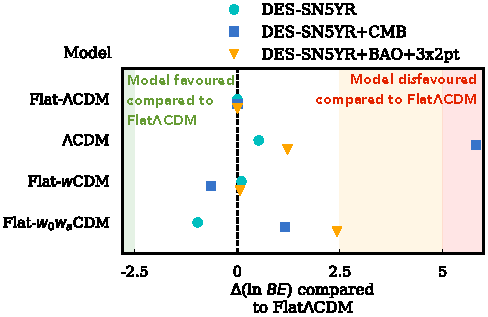
\includegraphics[width=0.5\textwidth]{figures/des_model_comparison.pdf}%
        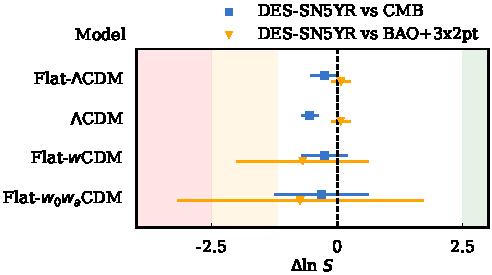
\includegraphics[width=0.5\textwidth]{figures/des_suspiciousness.pdf}
    \end{columns}
\end{frame}


\begin{frame}
    \frametitle{What is Nested Sampling?}
    \begin{itemize}
        \item Nested sampling is a radical, multi-purpose numerical tool.
        \item Given a (scalar) function $f$ with a vector of parameters $\theta$, it can be used for:
    \end{itemize}
    \vspace{-10pt}
    \begin{columns}[t]
        \column{0.3\textwidth}
        \begin{block}{Optimisation}
            \[\theta_\text{max} = \max_\theta{f(\theta)}\]
        \end{block}
        \column{0.3\textwidth}
        \begin{block}{Exploration}
            \vspace{-10pt}
            \[\text{draw/sample}\quad \theta\sim f\]
            \vspace{-15pt}
        \end{block}
        \column{0.3\textwidth}
        \begin{block}{Integration}
            \[\int f(\theta) dV \]
        \end{block}
    \end{columns}
    \begin{columns}[t]
        \column{0.33\textwidth}
        \centerline{\includegraphics[width=0.8\textwidth,page=13]{figures/himmelblau}}
        \column{0.33\textwidth}
        \centerline{\includegraphics[width=0.8\textwidth,page=15]{figures/himmelblau}}
        \column{0.33\textwidth}
        \centerline{\includegraphics[width=0.8\textwidth,page=14]{figures/himmelblau}}
    \end{columns}
\end{frame}

\begin{frame}
    \frametitle{Where is Nested Sampling?}
    \begin{columns}
        \column{0.5\textwidth}
        \begin{itemize}
            \item For many purposes, in your Neural Net you should group Nested Sampling with (MCMC) techniques such as:
                \begin{itemize}
                    \item Metropolis-Hastings (PyMC, MontePython)
                    \item Hamiltonian Monte Carlo (Stan, blackjax)
                    \item Ensemble sampling (emcee, zeus). 
                    \item Variational Inference (Pyro)
                    \item Sequential Monte Carlo 
                    \item Thermodynamic integration
                    \item Genetic algorithms
                \end{itemize}
            \item You may have heard of it branded form:
                \begin{itemize}
                    \item MultiNest
                    \item PolyChord
                    \item dynesty
                    \item ultranest
                \end{itemize}
            \end{itemize}
        \column{0.5\textwidth}
        \begin{columns}
            \column{0.5\textwidth}
        \includegraphics[width=\textwidth]{figures/emcee}
        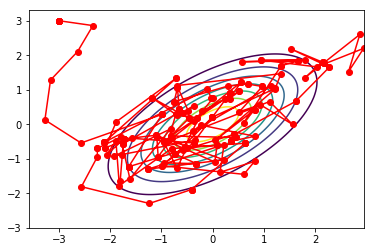
\includegraphics[width=\textwidth]{figures/metropolis-hastings}
            \column{0.5\textwidth}
        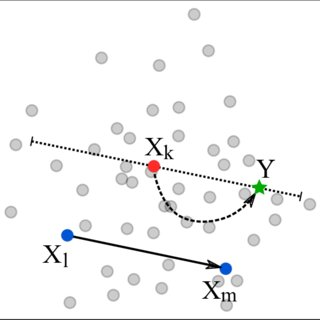
\includegraphics[width=\textwidth]{figures/zeus}
        \end{columns}
        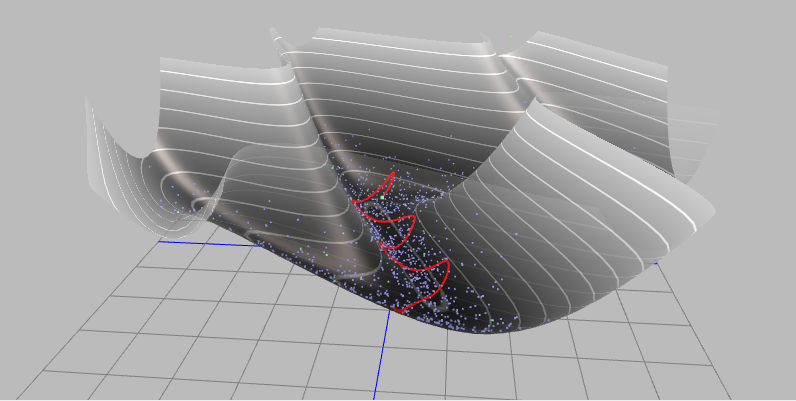
\includegraphics[width=\textwidth]{figures/hmc_explained}
    \end{columns}
\end{frame}

\begin{frame}
    \frametitle{Integration in Physics}
    \begin{itemize}
        \item Integration is a fundamental concept in physics, statistics and data science:
    \end{itemize}
    \begin{columns}
        \column{0.3\textwidth}
        \begin{block}{Partition functions}
            \vspace{-11pt}
            \[ Z(\beta) = \int e^{-\beta H(q,p)} dq dp \]
        \end{block}
        \column{0.3\textwidth}
        \begin{block}{Path integrals}
            \[ \Psi = \int e^{i S} \mathcal{D}x \]
        \end{block}
        \column{0.3\textwidth}
        \begin{block}{Bayesian marginals}
            \vspace{-11pt}
            \[ \mathcal{Z}(D) = \int \mathcal{L}(D|\theta) \pi(\theta) d\theta \]
        \end{block}
    \end{columns}
    \begin{columns}
        \column{0.6\textwidth}
        \begin{itemize}
            \item Need numerical tools if analytic solution unavailable.
            \item High-dimensional numerical integration is hard.
            \item Riemannian strategy estimates volumes geometrically:
                \[ \int f(x) d^nx \approx \sum_i f(x_i) \Delta V_i \sim \mathcal{O}(e^n) \]
            \item Curse of dimensionality $\Rightarrow$ exponential scaling.
        \end{itemize}
        \column{0.4\textwidth}
        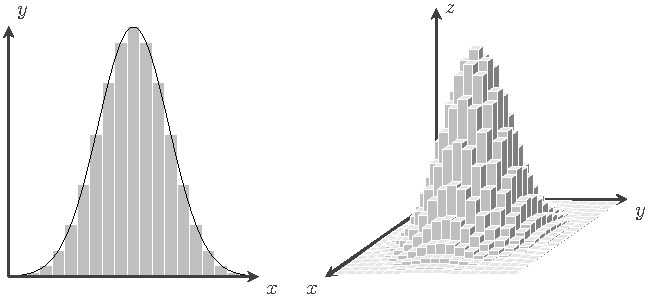
\includegraphics[width=\textwidth]{figures/integration.pdf}
    \end{columns}
\end{frame}

\begin{frame}
    \begin{columns}
        \column{0.48\textwidth}
        \begin{block}{\textbf{MCMC}}
            \only<16>{
                \begin{itemize}
                    \item Single ``walker''
                    \item Explores posterior
                    \item Fast, if proposal matrix is tuned
                    \item Parameter estimation, suspiciousness calculation
                    \item Channel capacity optimised for generating posterior samples
                \end{itemize}
            }
        \end{block}
            \includegraphics<1>[width=\textwidth,page=16]{figures/himmelblau}%
            \includegraphics<2>[width=\textwidth,page=17]{figures/himmelblau}%
            \includegraphics<3>[width=\textwidth,page=18]{figures/himmelblau}%
            \includegraphics<4>[width=\textwidth,page=19]{figures/himmelblau}%
            \includegraphics<5>[width=\textwidth,page=20]{figures/himmelblau}%
            \includegraphics<6-15>[width=\textwidth,page=21]{figures/himmelblau}%
        \centerline{\includegraphics<16>[width=0.5\textwidth,page=19]{figures/himmelblau}}
        \column{0.48\textwidth}
        \begin{block}<7->{\textbf{Nested sampling}}
            \only<16>{
                \begin{itemize}
                    \item Ensemble of ``live points''
                    \item Scans from prior to peak of likelihood
                    \item Slower, no tuning required
                    \item Parameter estimation, model comparison, tension quantification
                    \item Channel capacity optimised for computing partition function
                \end{itemize}
            }
        \end{block}
            \includegraphics<7|handout:0>[width=\textwidth,page=1]{figures/himmelblau}%
            \includegraphics<8|handout:0>[width=\textwidth,page=2]{figures/himmelblau}%
            \includegraphics<9|handout:0>[width=\textwidth,page=3]{figures/himmelblau}%
            \includegraphics<10          >[width=\textwidth,page=4]{figures/himmelblau}%
            \includegraphics<11|handout:0>[width=\textwidth,page=5]{figures/himmelblau}%
            \includegraphics<12|handout:0>[width=\textwidth,page=6]{figures/himmelblau}%
            \includegraphics<13|handout:0>[width=\textwidth,page=7]{figures/himmelblau}%
            \includegraphics<14|handout:0>[width=\textwidth,page=8]{figures/himmelblau}%
            \includegraphics<15|handout:0>[width=\textwidth,page=15]{figures/himmelblau}%
        \centerline{\includegraphics<16>[width=0.5\textwidth,page=4]{figures/himmelblau}} 
    \end{columns}
\end{frame}

\begin{frame}
    \frametitle{The nested sampling meta-algorithm: live points}
    \begin{columns}
        \column{0.5\textwidth}
        \begin{itemize}
            \item Start with $n$ random samples over the space.
            \item Delete outermost sample, and replace with a new random one at higher integrand value.
            \item The ``live points'' steadily contract around the peak(s) of the function.
            \item We can use this evolution to estimate volume \emph{probabilistically}.
            \item At each iteration, the contours contract by $\sim\frac{1}{n}\only<5->{\pm \frac{1}{n}}$ of their volume.
            \item This is an exponential contraction, so
                \[  \int f(x) dV \approx \sum_i f(x_i) \Delta V_i, \quad V_i = V_0 e^{-\only<5->{(}i\only<5->{\pm\sqrt{i})}/n} \]
%            \item Nested sampling: completely different way to scan.
%            \item Ensemble sampling compresses entire space$\to$peak(s).
%            \item Sequentially update a set $S$ of $n$ samples:
%                \begin{itemize}
%                    \item[$S_0$:]  Generate $n$ samples uniformly over the space (from a measure $\pi$). 
%
%                    \item[$S_{i+1}$:] Delete the lowest likelihood sample in $S_{i}$, and replace it with a new uniform sample with higher likelihood.
%                \end{itemize}
%            \item Requires one to be able to sample uniformly within a region, subject to a {\em hard constraint}:
%                \[\{\theta\sim \pi : \mathcal{L}(\theta)>\mathcal{L}_*. \}\]
%            \item This procedure optimises (multimodally), and can calculate the \C[3]{evidence}/integral of function \& \C[0]{posterior}/sample weights.
        \end{itemize}
        \column{0.5\textwidth}
        \includegraphics<1|handout:0>[width=\textwidth,page=1]{figures/himmelblau}%
        \includegraphics<2|handout:0>[width=\textwidth,page=2]{figures/himmelblau}%
        \includegraphics<3|handout:0>[width=\textwidth,page=3]{figures/himmelblau}%
        \includegraphics<4-         >[width=\textwidth,page=4]{figures/himmelblau}%
    \end{columns}
\end{frame}

\begin{frame}
    \frametitle{The nested sampling meta-algorithm: dead points}
    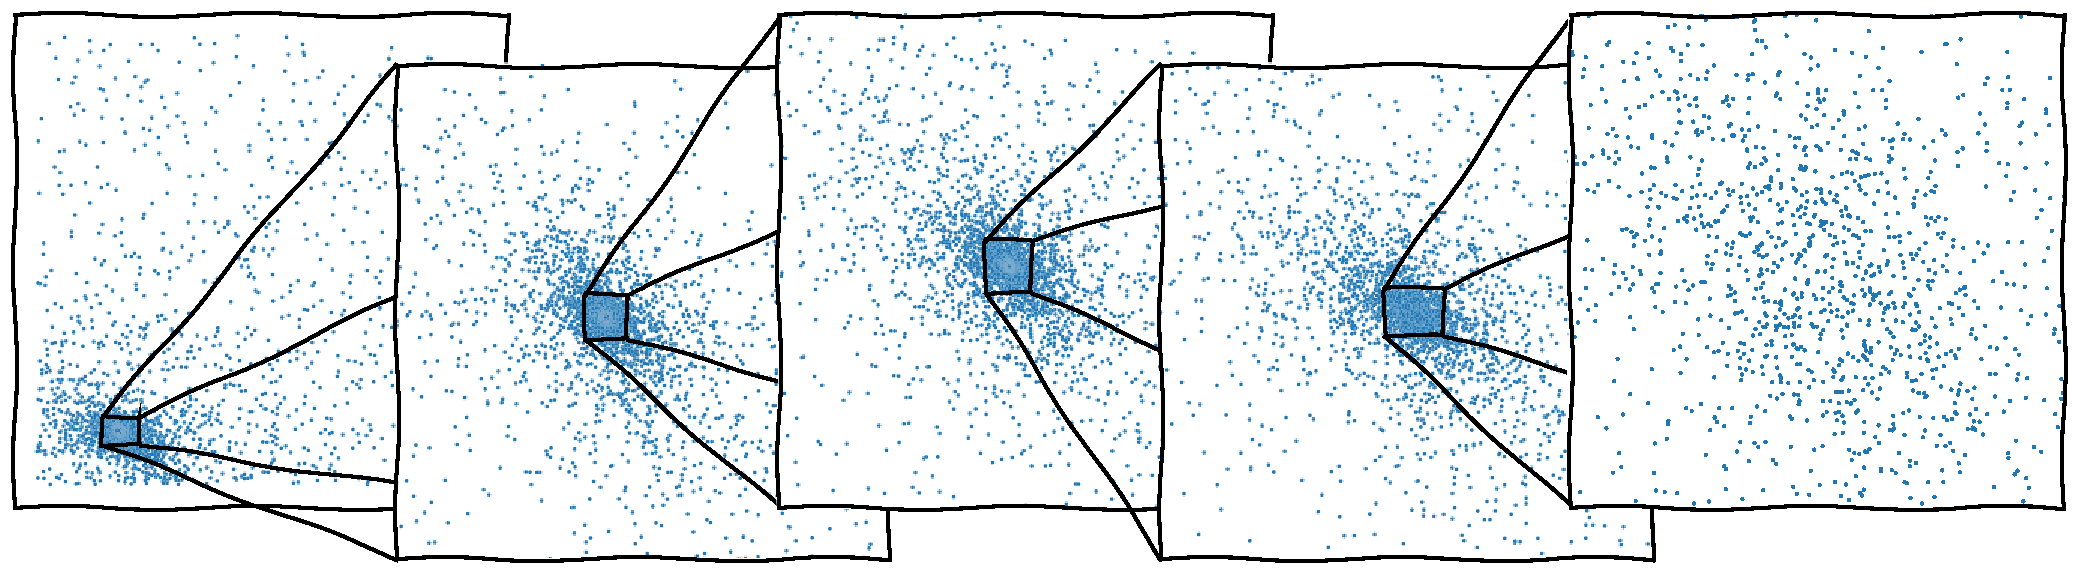
\includegraphics[width=\textwidth]{figures/dead_measure}
    \begin{columns}
        \column{0.69\textwidth}
        \begin{itemize}
            \item At the end, one is left with a set of discarded ``dead'' points.
            \item Dead points have a unique scale-invariant distribution $\propto\: \tfrac{dV}{V}$.
            \item Uniform over original region, exponentially concentrating on region of interest (until termination volume).
            \item Good for training emulators (HERA~\arxiv{2108.07282}).
        \end{itemize}
        \column{0.3\textwidth}
        \begin{block}{Applications}
        \begin{itemize}
            \item training emulators.
            \item gridding simulations
            \item beta flows
            \item ``dead measure'' 
        \end{itemize}
        \end{block}
    \end{columns}
\end{frame}

\begin{frame}
    \frametitle{Implementations of Nested Sampling \arxiv{2205.15570}(NatReview)}
    %\begin{columns}
    %    \begin{column}{0.33}
    %        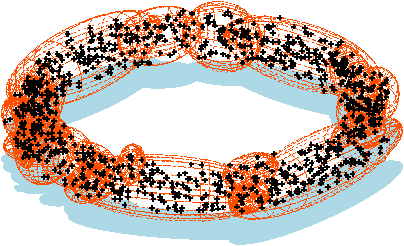
\includegraphics[width=\textwidth]{figures/multinest}
    %    \end{column} 
    %\end{columns}
    \begin{columns}[t]
        \column{0.3\textwidth}
        \texttt{MultiNest}~\arxiv{0809.3437}
        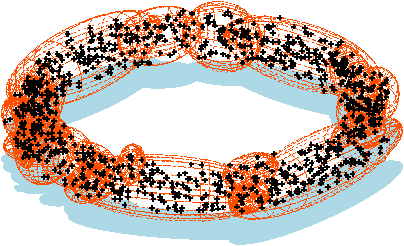
\includegraphics[width=\textwidth]{figures/multinest}
        \texttt{UltraNest}~\arxiv{2101.09604}
        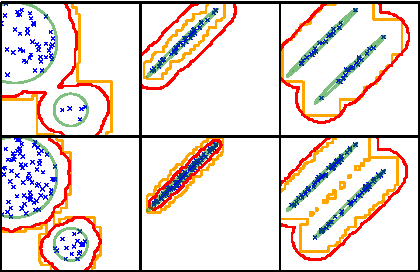
\includegraphics[width=\textwidth]{figures/radfriends}
        \texttt{nautilus}~\arxiv{2306.16923} 
        \column{0.4\textwidth}
        \texttt{PolyChord}~\arxiv{1506.00171}
        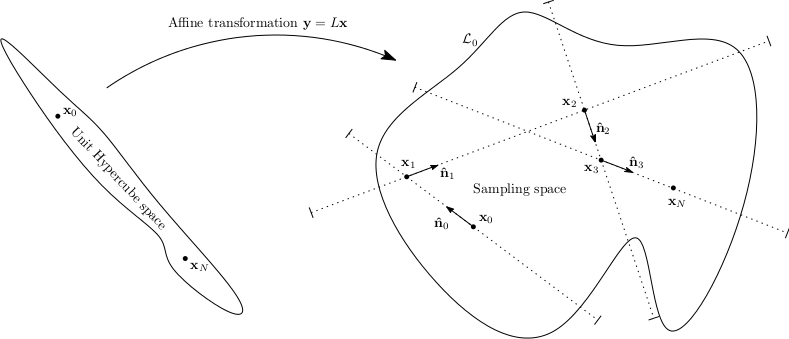
\includegraphics[width=\textwidth]{figures/polychord}
        \vfill
        \texttt{NeuralNest}~\arxiv{1903.10860}
        \begin{columns}
            \column{0.55\textwidth}
            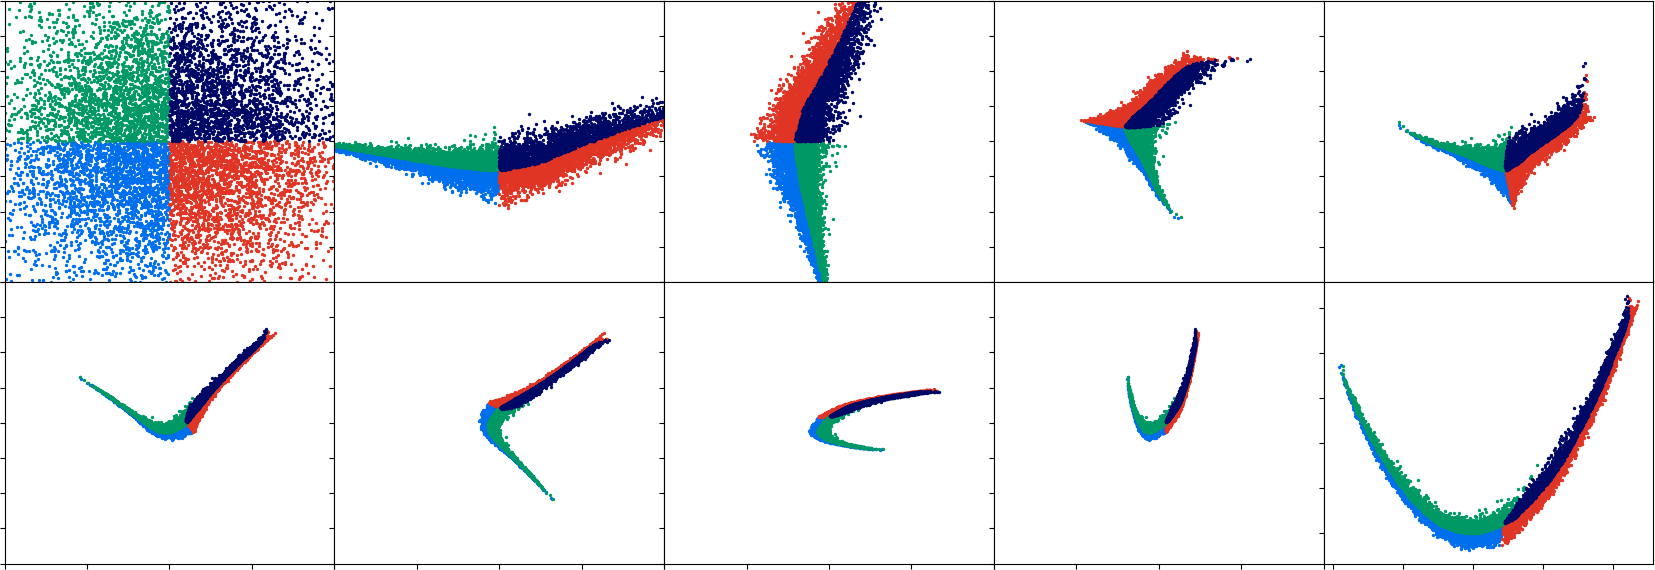
\includegraphics[width=\textwidth]{figures/rosenbrock_flow.png}
            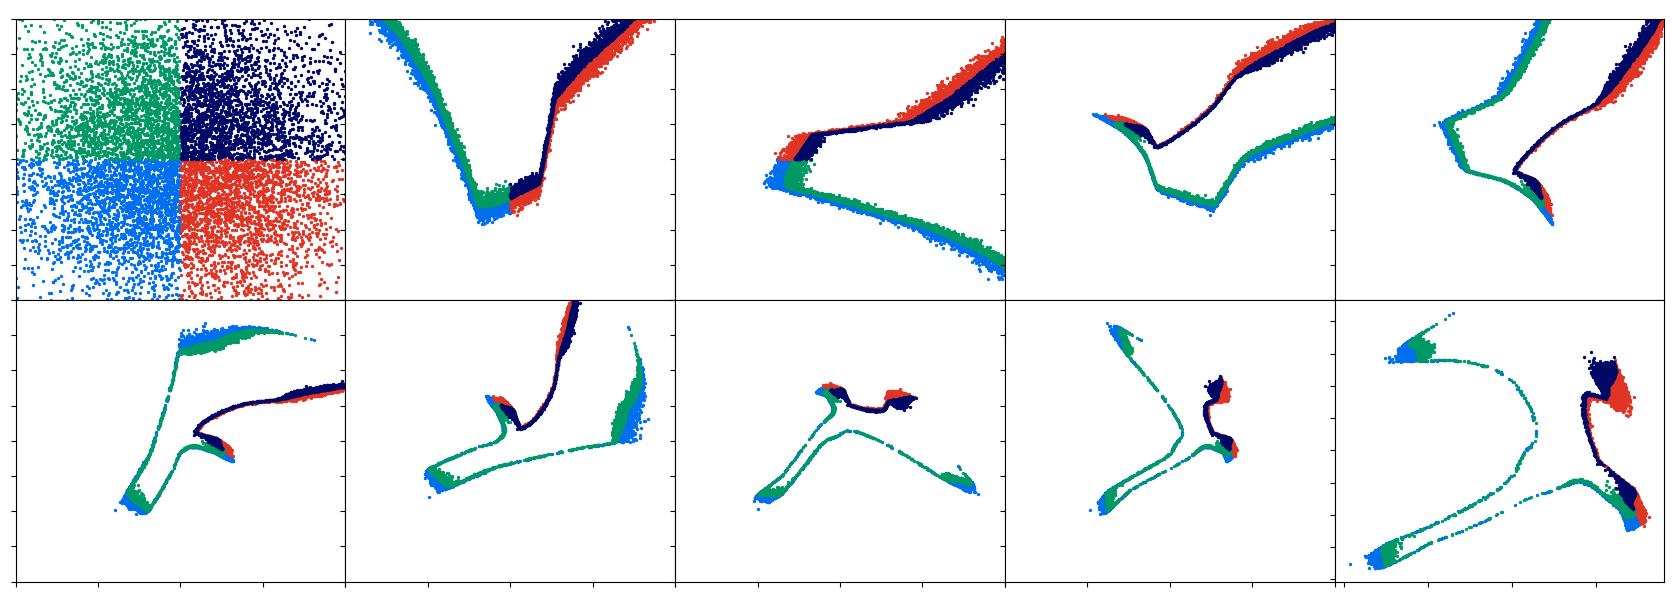
\includegraphics[width=\textwidth]{figures/himmelblau_flow.png}
            \column{0.45\textwidth}
            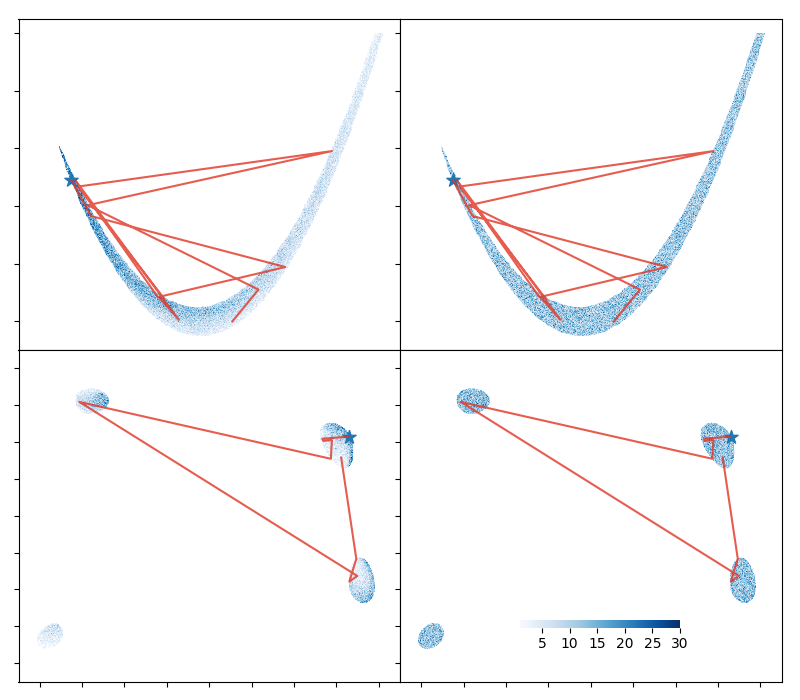
\includegraphics[width=\textwidth]{figures/chains.png}
        \end{columns}
        \texttt{nessai}~\arxiv{2102.11056} \texttt{nora}~\arxiv{2305.19267} \texttt{jaxnest}~\arxiv{2012.15286}
        \vfill
        \column{0.3\textwidth}
        \texttt{DNest}~\arxiv{1606.03757}
        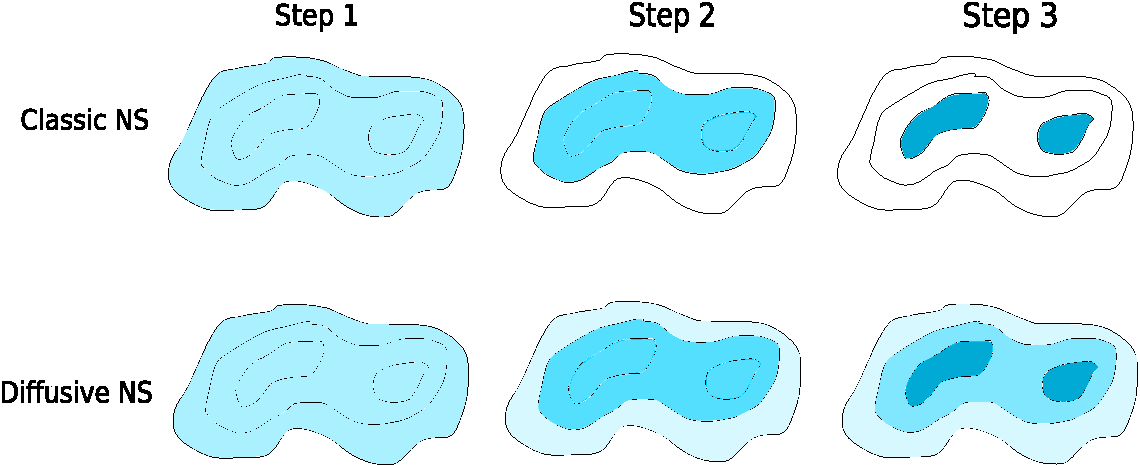
\includegraphics[width=\textwidth]{figures/dnest}
        \texttt{ProxNest}~\arxiv{2106.03646}
        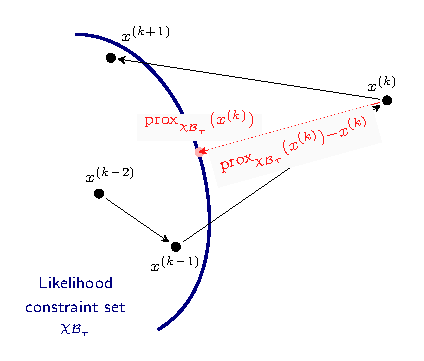
\includegraphics[width=\textwidth]{figures/proxnest_diagram}
        \texttt{dynesty}~\arxiv{1904.02180} 
        \vfill
    \end{columns}
\end{frame}

\begin{frame}
    \frametitle{Types of nested sampler}
    \begin{itemize}
        \item Broadly, most nested samplers can be split into how they create new live points.
        \item i.e. how they sample from the hard likelihood constraint $\{\theta\sim \pi : \mathcal{L}(\theta)>\mathcal{L}_* \}$.
    \end{itemize}
    \vspace{-10pt}
    \begin{columns}[t]
        \column{0.48\textwidth}
        \begin{block}{Rejection samplers}
            \begin{itemize}
                \item e.g. \texttt{MultiNest}, \texttt{UltraNest}.
\item Constructs bounding region and draws many invalid points until $\mathcal{L}(\theta)>\mathcal{L}_*$.
                \item Efficient in low dimensions, exponentially inefficient $\sim\mathcal{O}(e^{d/d_0})$ in high  $d>d_0\sim10$.
            \end{itemize}
        \end{block}
        \column{0.48\textwidth}
        \begin{block}{Chain-based samplers}
            \begin{itemize}
                \item e.g. \texttt{PolyChord}, \texttt{ProxNest}.
                \item Run Markov chain starting at a live point, generating many valid (correlated) points.
                \item Linear $\sim\mathcal{O}(d)$ penalty in decorrelating new live point from the original seed point.
            \end{itemize}
        \end{block}
    \end{columns}
    \vspace{5pt}
    \begin{itemize}
        \item Nested samplers usually come with:
            \begin{itemize}
                \item \emph{resolution} parameter $n_\mathrm{live}$ (which improve results as $\sim\mathcal{O}(n_\mathrm{live}^{-1/2})$.
                    \item set of \emph{reliability} parameters~\arxiv{2101.04525}, which don't improve results if set arbitrarily high, but introduce systematic errors if set too low.
                    \item e.g. \texttt{Multinest} efficiency \texttt{eff} or \texttt{PolyChord} chain length $n_\mathrm{repeats}$.
            \end{itemize}
    \end{itemize}
\end{frame}

%\begin{frame}
%    \frametitle{Applications: The three pillars of Bayesian inference}
%    \begin{columns}[t]
%        \column{0.33\textwidth}
%        \begin{block}{Parameter estimation}
%            What do the data tell us about the parameters of a model?
%
%            \textit{e.g. the size or age of a $\Lambda$CDM universe}
%            \[ \hspace{-4pt}\C[0]{P(\theta|D,M)} = \frac{\C[2]{P(D|\theta,M)} \C[1]{P(\theta|M)}}{\C[3]{P(D|M)}} \] 
%            \[ \C[0]{\mathcal{P}} = \frac{\C[2]{\mathcal{L}} \times\C[1]{\pi}}{\C[3]{\mathcal{Z}}}\] 
%            \[ \C[0]{\text{Posterior}} = \frac{\C[2]{\text{Likelihood}} \times\C[1]{\text{Prior}}}{\C[3]{\text{Evidence}}}\]
%        \end{block}
%        \column{0.3\textwidth}
%        \begin{block}{Model comparison}
%            How much does the data support a particular model?
%
%            \textit{e.g. $\Lambda$CDM vs a dynamic dark energy cosmology}
%            \[ \C[4]{P(M|D)} = \frac{\C[3]{P(D|M)} \C[5]{P(M)}}{\C[7]{P(D)}} \vspace{-7pt}\]
%            \[ \frac{\C[3]{\mathcal{Z}_\mathcal{M}} \C[5]{\Pi_\mathcal{M}}}{\C[7]{\sum_m Z_m \Pi_m}} \]
%            \[ \C[4]{\text{Posterior}} = \frac{\C[3]{\text{Evidence}} \times\C[5]{\text{Prior}}}{\C[7]{\text{Normalisation}}}\]
%        \end{block}
%        \column{0.33\textwidth}
%        \begin{block}{Tension quantification}
%            Do different datasets make consistent predictions from the same model? 
%            \textit{e.g. CMB vs Type IA supernovae data}
%            \[ \mathcal{R} = \frac{\C[3]{\mathcal{Z}}_{AB}}{\C[3]{\mathcal{Z}}_A\C[3]{\mathcal{Z}}_\mathcal{B}}\] 
%            \[
%                \begin{aligned} \log\mathcal{S} = \av[{\C[0]{\mathcal{P}}_{AB}}]{\C[2]{\log\mathcal{L}}_{AB}}&\\
%                    -\av[{\C[0]{\mathcal{P}}_{A}}]{\C[2]{\log\mathcal{L}}_{A}}&\\
%                    -\av[{\C[0]{\mathcal{P}}_{B}}]{\C[2]{\log\mathcal{L}}_{B}}&
%                \end{aligned}
%            \]
%        \end{block}
%    \end{columns}
%\end{frame}

\begin{frame}
    \frametitle{Applications of nested sampling}
    \framesubtitle{Cosmology}
    \student{adam_ormondroyd}{Adam Ormondroyd}{PhD}
    \begin{columns}
        \column{0.55\textwidth}
        \begin{itemize}
            \item Battle-tested in Bayesian cosmology on
                \begin{itemize}
                    \item Parameter estimation: multimodal alternative to MCMC samplers.
                    \item Model comparison: using integration to compute the Bayesian evidence
                    \item Tension quantification: using deep tail sampling and suspiciousness computations.
                \end{itemize}
            \item Plays a critical role in major cosmology pipelines: Planck, DES, KiDS, BAO, SNe.
            \item The default $\Lambda$CDM cosmology is well-tuned to have Gaussian-like posteriors for CMB data. 
            \item Less true for alternative cosmologies/models and orthogonal datasets, so nested sampling crucial.
        \end{itemize}
        \column{0.45\textwidth}
        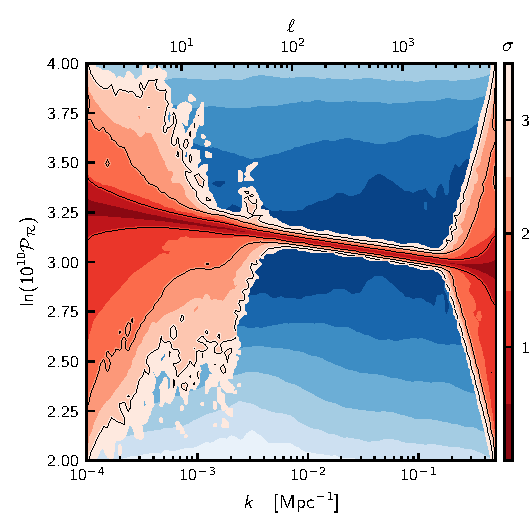
\includegraphics[width=0.49\textwidth]{figures/pps_both}
        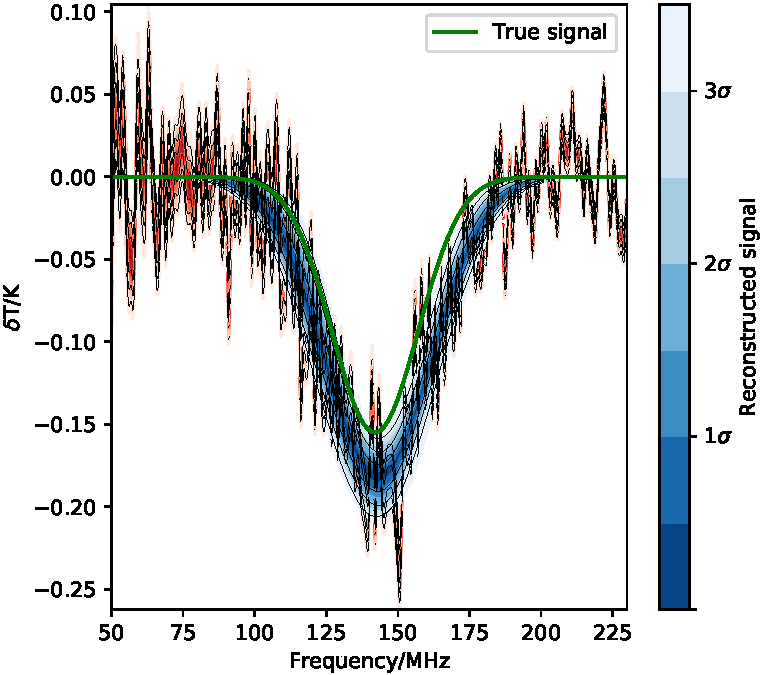
\includegraphics[width=0.49\textwidth]{figures/reach_fit-cropped.pdf}
        %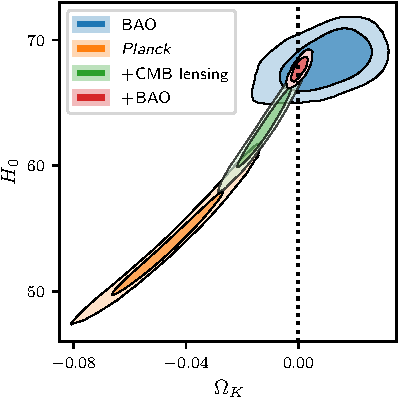
\includegraphics[width=0.49\textwidth]{figures/curvature_3}
        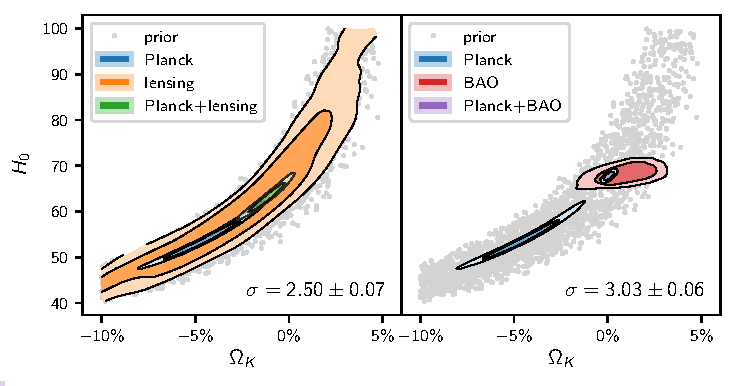
\includegraphics[width=\textwidth]{figures/omegak_H0_2.pdf}
    \end{columns}
\end{frame}

\begin{frame}
    \frametitle{Applications of nested sampling}
    \framesubtitle{Astrophysics}
\student{metha_prathaban}{Metha Prathaban}{PhD}
    \begin{columns}
        \column{0.6\textwidth}
        \begin{itemize}
            \item In exoplanets~\arxiv{1806.00518}
                \begin{itemize}
                    \item Parameter estimation: determining properties of planets.
                    \item Model comparison: how many planets? Stellar modelling~\arxiv{2007.07278}.
                    \item exoplanet problems regularly have posterior phase transitions \arxiv{2102.03387}
                \end{itemize}
            \item In gravitational waves
                \begin{itemize}
                    \item Parameter estimation: Binary merger properties
                    \item Model comparison: Modified theories of gravity, selecting phenomenological parameterisations~\arxiv{1803.10210}
                    \item Likelihood reweighting: fast slow properties
                \end{itemize}
        \end{itemize}
        \column{0.4\textwidth}
        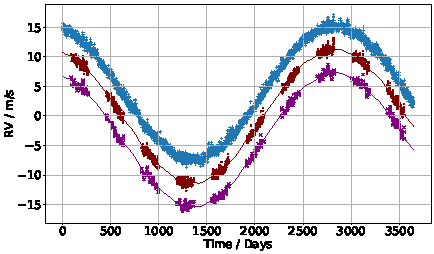
\includegraphics[width=\textwidth]{figures/rv_full.pdf}
        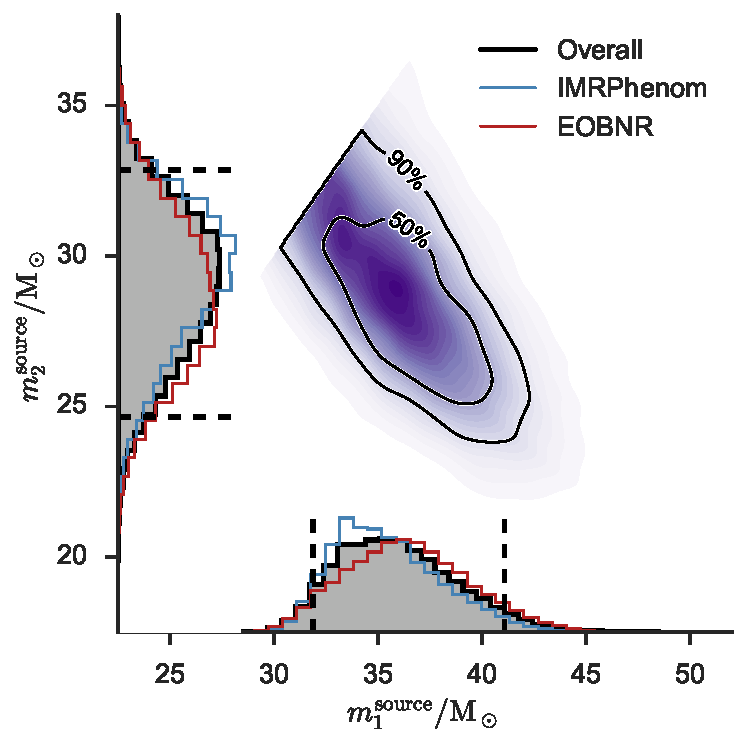
\includegraphics[width=0.49\textwidth]{figures/ligo_m1_m2.pdf}
        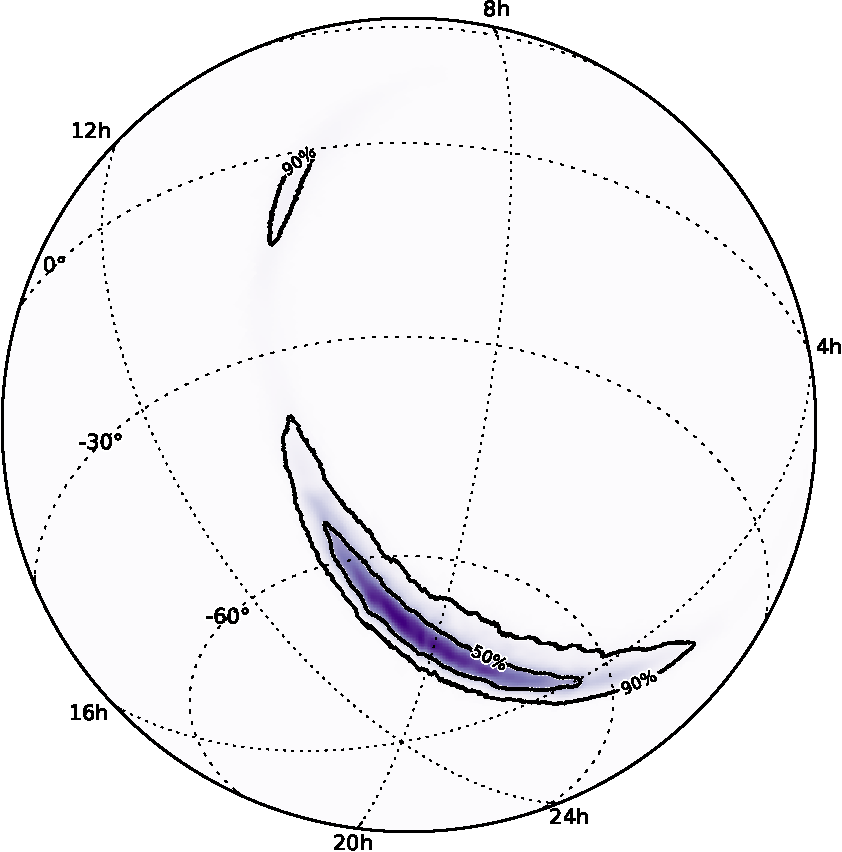
\includegraphics[width=0.49\textwidth]{figures/ligo_lambert-skymap.pdf}
    \end{columns}
\end{frame}

\begin{frame}
    \frametitle{Applications of nested sampling}
    \framesubtitle{Particle physics}
    \student{david_yallup}{David Yallup}{PDRA}
    \begin{columns}
        \column{0.56\textwidth}
        \begin{columns}
            \column{0.67\textwidth}
            \begin{itemize}
                \item Nested sampling for cross section computation/event generation
            \end{itemize}
            \column{0.3\textwidth}
            \[\sigma = \int_\Omega d\Phi |\mathcal{M}|^2.\]
        \end{columns}
        \begin{itemize}
            \item Nested sampling can explore the phase space $\Omega$ and compute integral blind with comparable efficiency to HAAG/RAMBO~\arxiv{2205.02030}.
            \item Bayesian sparse reconstruction~\arxiv{1809.04598} applied to bump hunting allows evidence-based detection of signals in phenomenological backgrounds~\arxiv{2211.10391}.
            \item Fine tuning quantification
            \item Fast estimation of small $p$-values \arxiv{2106.02056}(PRL), just make switch:\\ $X\leftrightarrow p$, $\mathcal{L}\leftrightarrow\lambda$, $\theta \leftrightarrow x$.

        \end{itemize}
        \column{0.17\textwidth}
        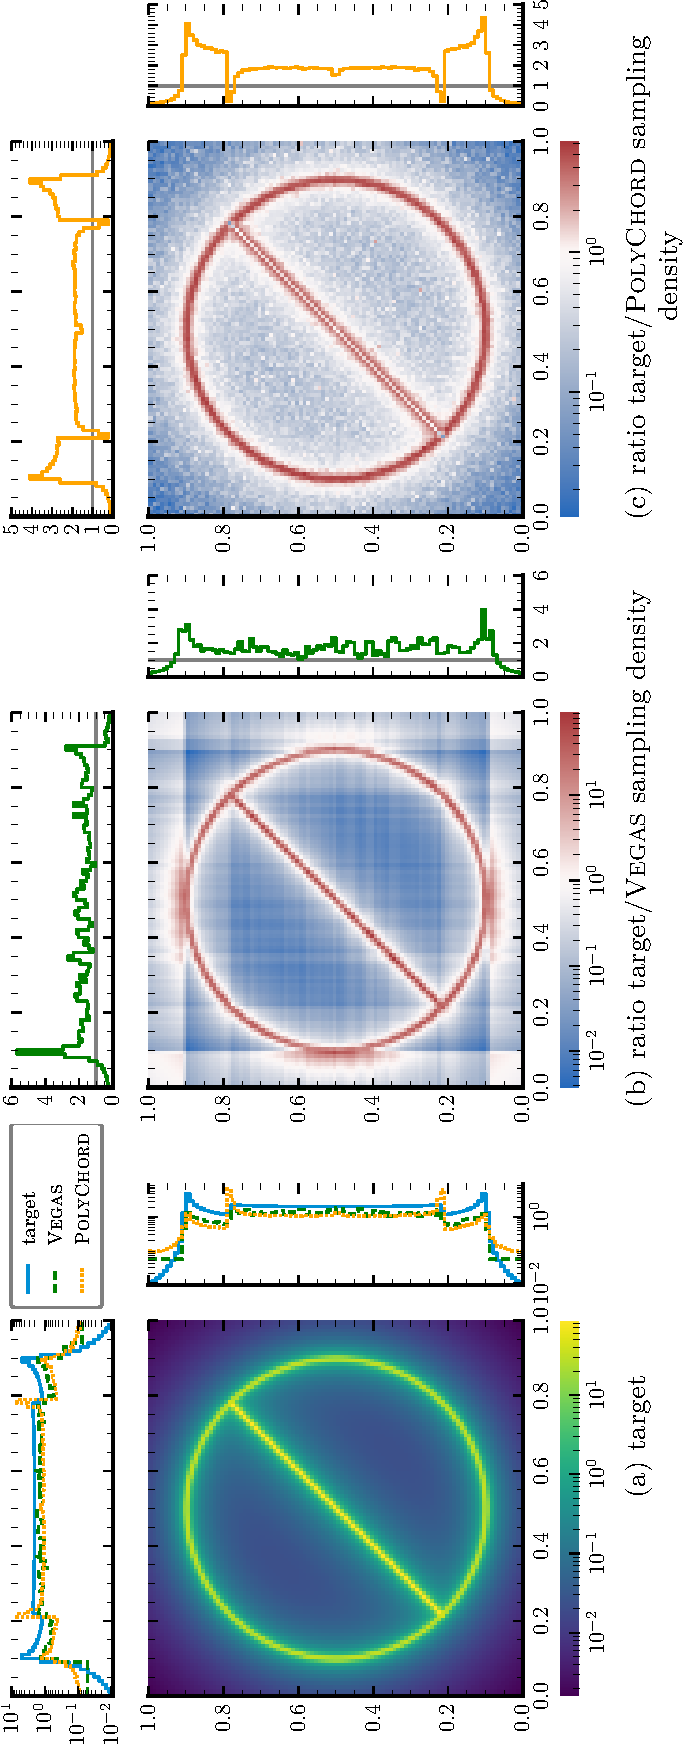
\includegraphics[width=\textwidth]{figures/phase_space_1-pdfjam-crop.pdf}
        \column{0.27\textwidth}
        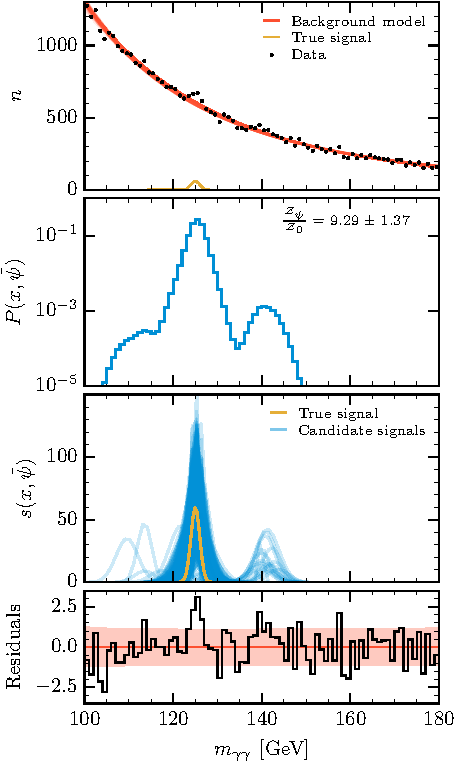
\includegraphics[width=\textwidth]{figures/psi_predict-crop.pdf}
    \end{columns}
\end{frame}


\begin{frame}
    \frametitle{Applications of nested sampling}
    \framesubtitle{Lattice field theory}
\student{david_yallup}{David Yallup}{PDRA}
    \begin{columns}
        \column{0.5\textwidth}
        \begin{itemize}
            \item Consider standard field theory Lagrangian:
                \[ Z(\beta) = \int D\phi e^{-\beta S(\phi)}, \quad S(\phi) = \int dx^\mu \mathcal{L}(\phi) \]
            \item Discretize onto spacetime grid.
            \item Compute partition function
            \item NS unique traits:
                \begin{itemize}
                    \item Get full partition function for free
                    \item allows for critical tuning
                    \item avoids critical slowing down
                \end{itemize}
            \item Applications in lattice gravity, QCD, condensed matter physics
        \end{itemize}
        \column{0.5\textwidth}
        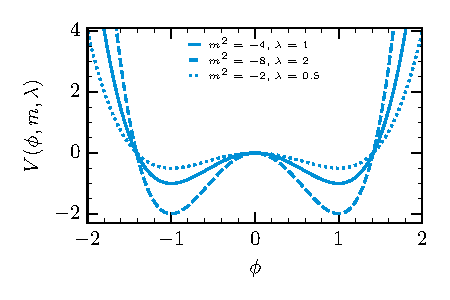
\includegraphics[width=0.49\textwidth]{figures/potential_shape}
        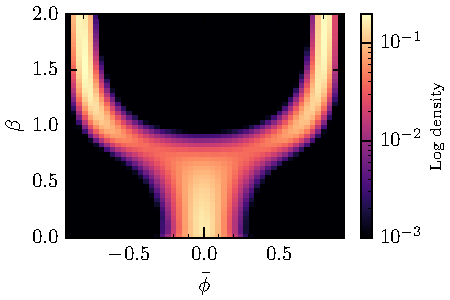
\includegraphics[width=0.49\textwidth]{figures/2d_phase}
        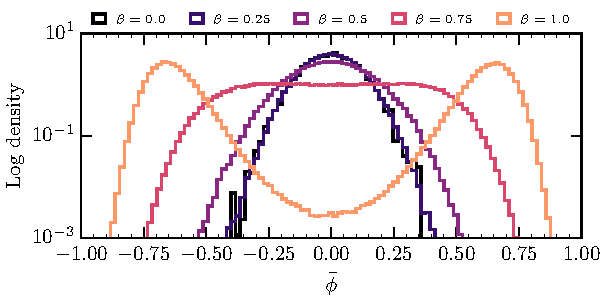
\includegraphics[width=\textwidth]{figures/lattice_field_theory.pdf}
    \end{columns}
\end{frame}
\begin{frame}
    \frametitle{Applications of nested sampling}
    \framesubtitle{Machine learning}
\student{kamran_javid}{Kamran Javid}{PDRA}
    \begin{columns}
        \column{0.62\textwidth}
        \begin{itemize}
            \item Machine learning requires:
                \begin{itemize}
                    \item Training to find weights
                    \item Choice of architecture/topology/hyperparameters
                \end{itemize}
            \item Bayesian NNs treat training as a model fitting problem
            \item Compute posterior of weights (parameter estimation), rather than optimisation (gradient descent)
            \item Use evidence to determine best architecture (model comparison), correlates with out-of-sample performance! 
            \item Solving the full ``shallow learning'' problem without compromise \arxiv{2004.12211}\arxiv{2211.10391}. 
                \begin{itemize}
                    \item Promising work ongoing to extend this to transfer learning and deep nets.
                \end{itemize}
            \item More generally, dead points are optimally spaced  for training traditional ML approaches e.g. \arxiv{2309.05697}
        \end{itemize}
        \column{0.38\textwidth}
        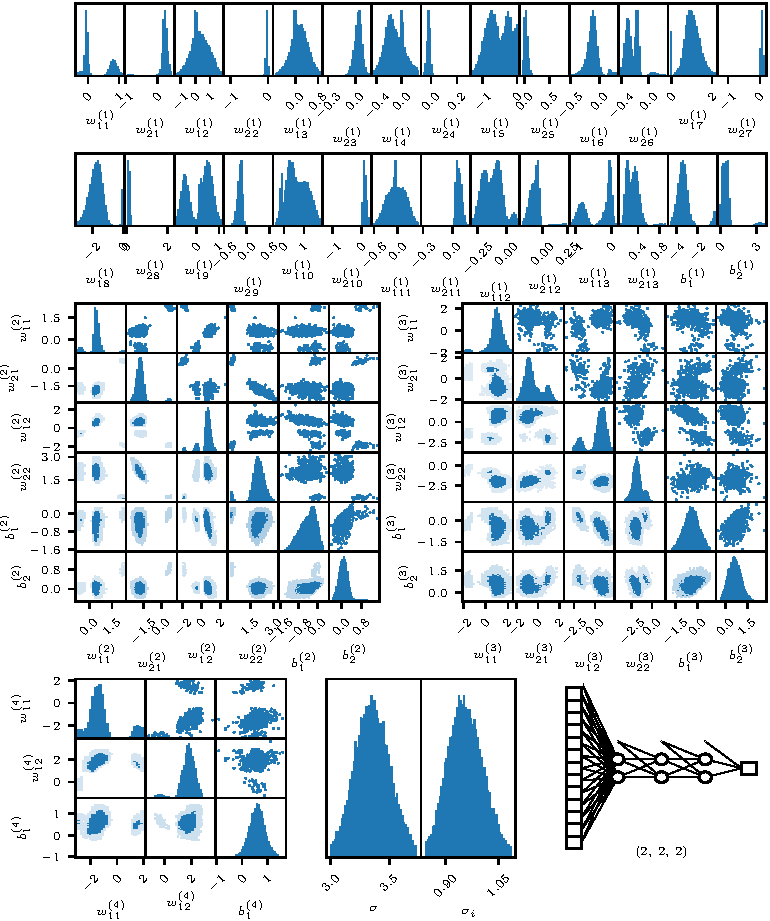
\includegraphics[width=\textwidth]{figures/nn_posterior-cropped.pdf}
    \end{columns}
\end{frame}

%\begin{frame}
%    \frametitle{Applications of nested sampling}
%    \framesubtitle{Statistics: fast estimation of small $p$-values~\arxiv{2106.02056}(PRL)}
%    \begin{columns}
%        \column{0.57\textwidth}
%        \begin{itemize}
%            \item Nested sampling for frequentist computation!?
%            \item $p$-value: $P(\lambda>\lambda^*|H_0)$ -- probability that test statistic $\lambda$ is at least as great as observed $\lambda^*$.
%            \item Computation of a tail probability from sampling distribution of $\lambda$ under $H_0$.
%            \item For gold-standard $5\sigma$, this is very expensive to simulate directly ($\sim10^9$ by definition).
%            \item Need insight/approximation to make efficient.
%            \item Nested sampling is tailor-made for this, just make switch: $X\leftrightarrow p$, $\mathcal{L}\leftrightarrow\lambda$, $\theta \leftrightarrow x$.
%            \item The only real conceptual shift is switching the integrator from parameter- to data-space.
%        \end{itemize}
%        \column{0.43\textwidth}
%        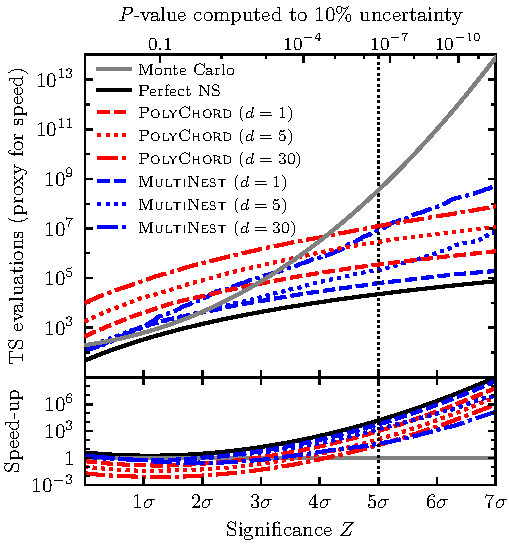
\includegraphics[width=\textwidth]{figures/pvalue.pdf}
%    \end{columns}
%\end{frame}

\begin{frame}
    \frametitle{Applications of nested sampling}
    \framesubtitle{And beyond\ldots}
    \only<1-4>{
        \student{watkinson-headshot}{Catherine Watkinson}{Senior Data Scientist}
    }
    \only<5->{
        \student{mcaloone-headshot}{Thomas Mcaloone}{PhD $\to$ Data Scientist}
    }
    \begin{columns}
        \column{0.6\textwidth}
        \begin{itemize}
            \item Techniques have been spun-out (PolyChord Ltd) to:
            \item Protein folding
                \begin{itemize}
                    \item Navigating free energy surface.
                    \item Computing misfolds.
                    \item Thermal motion.
                \end{itemize}
            \item Nuclear fusion reactor optimisation
                \begin{itemize}
                    \item multi-objective.
                    \item uncertainty propagation.
                \end{itemize}
            \item Telecoms \& DSTL research (MIDAS)
                \begin{itemize}
                    \item Optimising placement of transmitters/sensors.
                    \item Maximum information data acquisition strategies.
                \end{itemize}
        \end{itemize}
            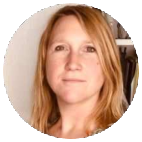
\includegraphics[width=0.08\textwidth]{figures/headshots/catherine-watkinson.pdf}%
            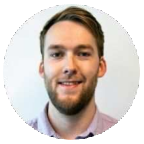
\includegraphics[width=0.08\textwidth]{figures/headshots/thomas-macaloone.pdf}%
            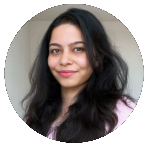
\includegraphics[width=0.08\textwidth]{figures/headshots/parul-janagal.pdf}%
            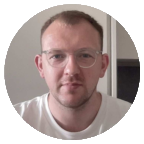
\includegraphics[width=0.08\textwidth]{figures/headshots/angus-peters.pdf}%
            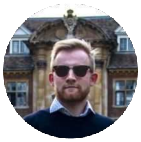
\includegraphics[width=0.08\textwidth]{figures/headshots/tamas-stenzel.pdf}%
            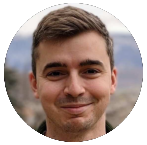
\includegraphics[width=0.08\textwidth]{figures/headshots/david-yallup.pdf}%
            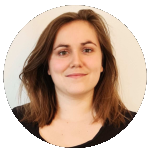
\includegraphics[width=0.08\textwidth]{figures/headshots/rebecca-handley.pdf}%
            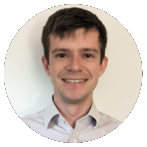
\includegraphics[width=0.08\textwidth]{figures/headshots/adam-ormondroyd.pdf}%
            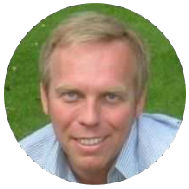
\includegraphics[width=0.08\textwidth]{figures/headshots/mike-hobson.pdf}%
            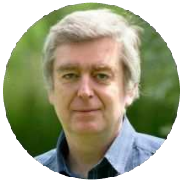
\includegraphics[width=0.08\textwidth]{figures/headshots/anthony-lasenby.pdf}%
            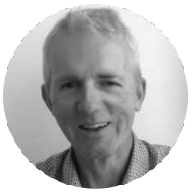
\includegraphics[width=0.08\textwidth]{figures/headshots/mike-handley.pdf}%
            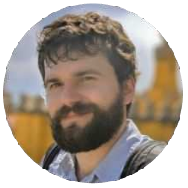
\includegraphics[width=0.08\textwidth]{figures/headshots/will-handley.pdf}%
        \column{0.4\textwidth}
        \includegraphics<1|handout:0>[width=\textwidth]{figures/protein_1.png}%
        \includegraphics<2          >[width=\textwidth]{figures/protein_2.png}%
        \includegraphics<3|handout:0>[width=\textwidth]{figures/protein_3.png}%
        \includegraphics<4|handout:0>[width=\textwidth]{figures/lcoe.png}%
        %\includegraphics<5|handout:0>[width=\textwidth]{figures/tdoa-cropped-1-crop.pdf}%
        %\includegraphics<6|handout:0>[width=\textwidth]{figures/tdoa-cropped-2-crop.pdf}%
        %\includegraphics<7|handout:0>[width=\textwidth]{figures/tdoa-cropped-3-crop.pdf}%
        \includegraphics<5|handout:0>[width=\textwidth]{figures/DKL_contour-cropped-crop.pdf}%
        \includegraphics<6|handout:0>[width=\textwidth]{figures/mean_DKL_optimise-3-crop.pdf}%
        \includegraphics<7|handout:0>[width=\textwidth]{figures/mean_DKL_optimise-4-crop.pdf}%
        \includegraphics<8|handout:0>[width=\textwidth]{figures/mean_DKL_optimise-5-crop.pdf}%
    \end{columns}
\end{frame}

\begin{frame}
    \frametitle{REACH: Global 21cm cosmology {\small \arxiv{2210.07409}(NatAstro)}}
    \student{ian_roque}{Ian Roque}{PhD}
    \vspace{10pt}
    \begin{columns}
        \column{0.65\textwidth}
        \vspace{-10pt}
        \begin{itemize}
            \item Imaging the universal dark ages using CMB backlight.
            \item $21\text{cm}$ hyperfine line emission from neutral hydrogen.
            \item Global experiments measure monopole across frequency.
            \item Challenge: science hidden in foregrounds $\sim 10^4\times$signal.
            \item Lead data analysis team (REACH first light in January)
            \item Nested sampling woven in from the ground up (calibrator, beam modelling, signal fitting, likelihood selection).
            \item All treated as parameterised model comparison problems.
        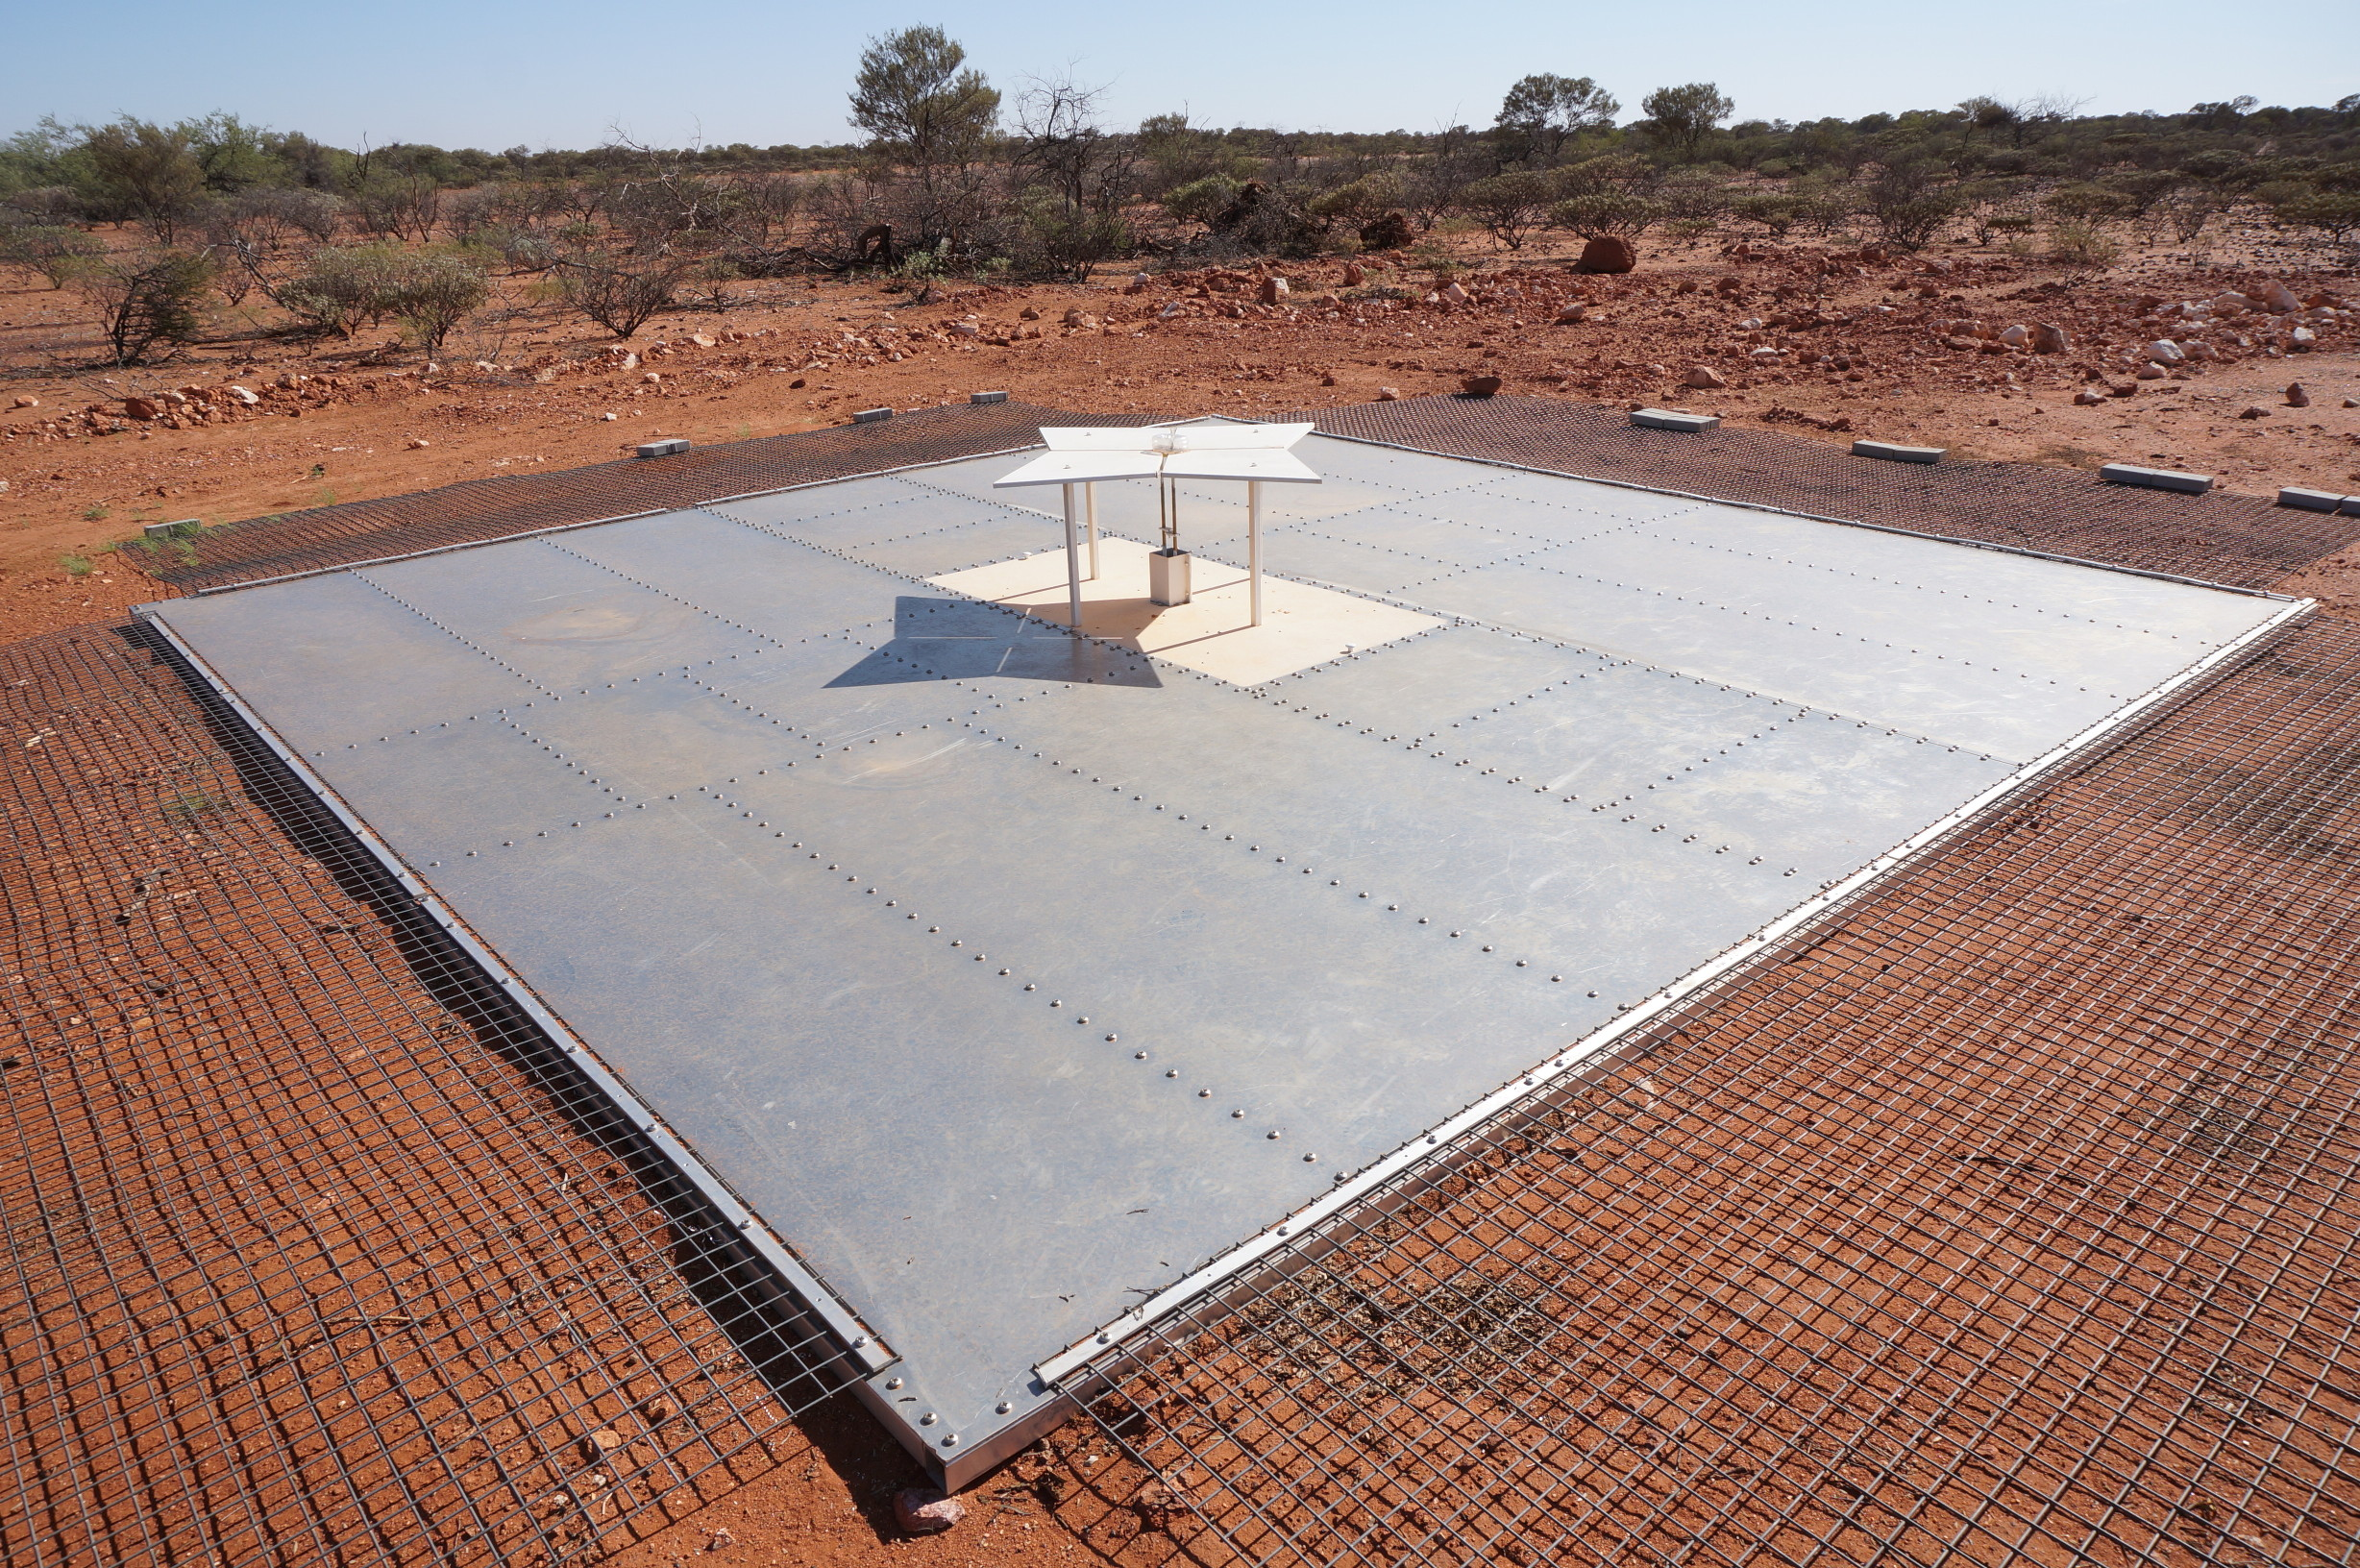
\includegraphics[height=0.3\textwidth]{figures/EDGES_antenna}
        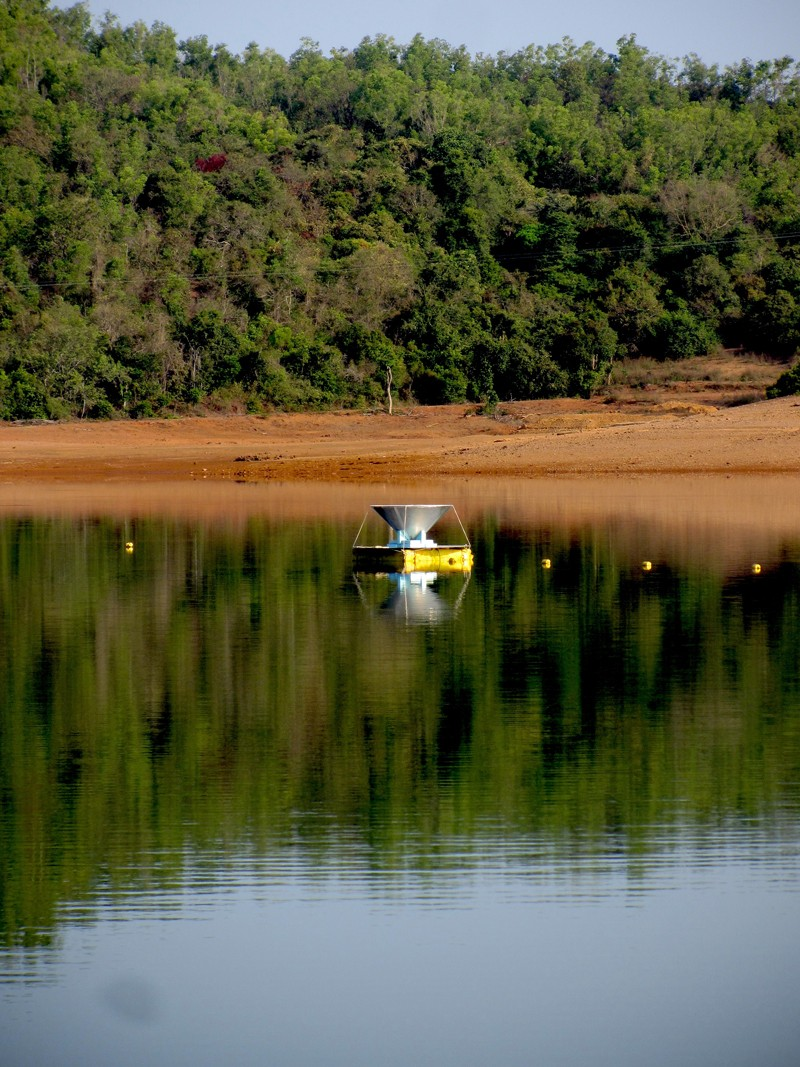
\includegraphics[height=0.3\textwidth]{figures/SARAS}
        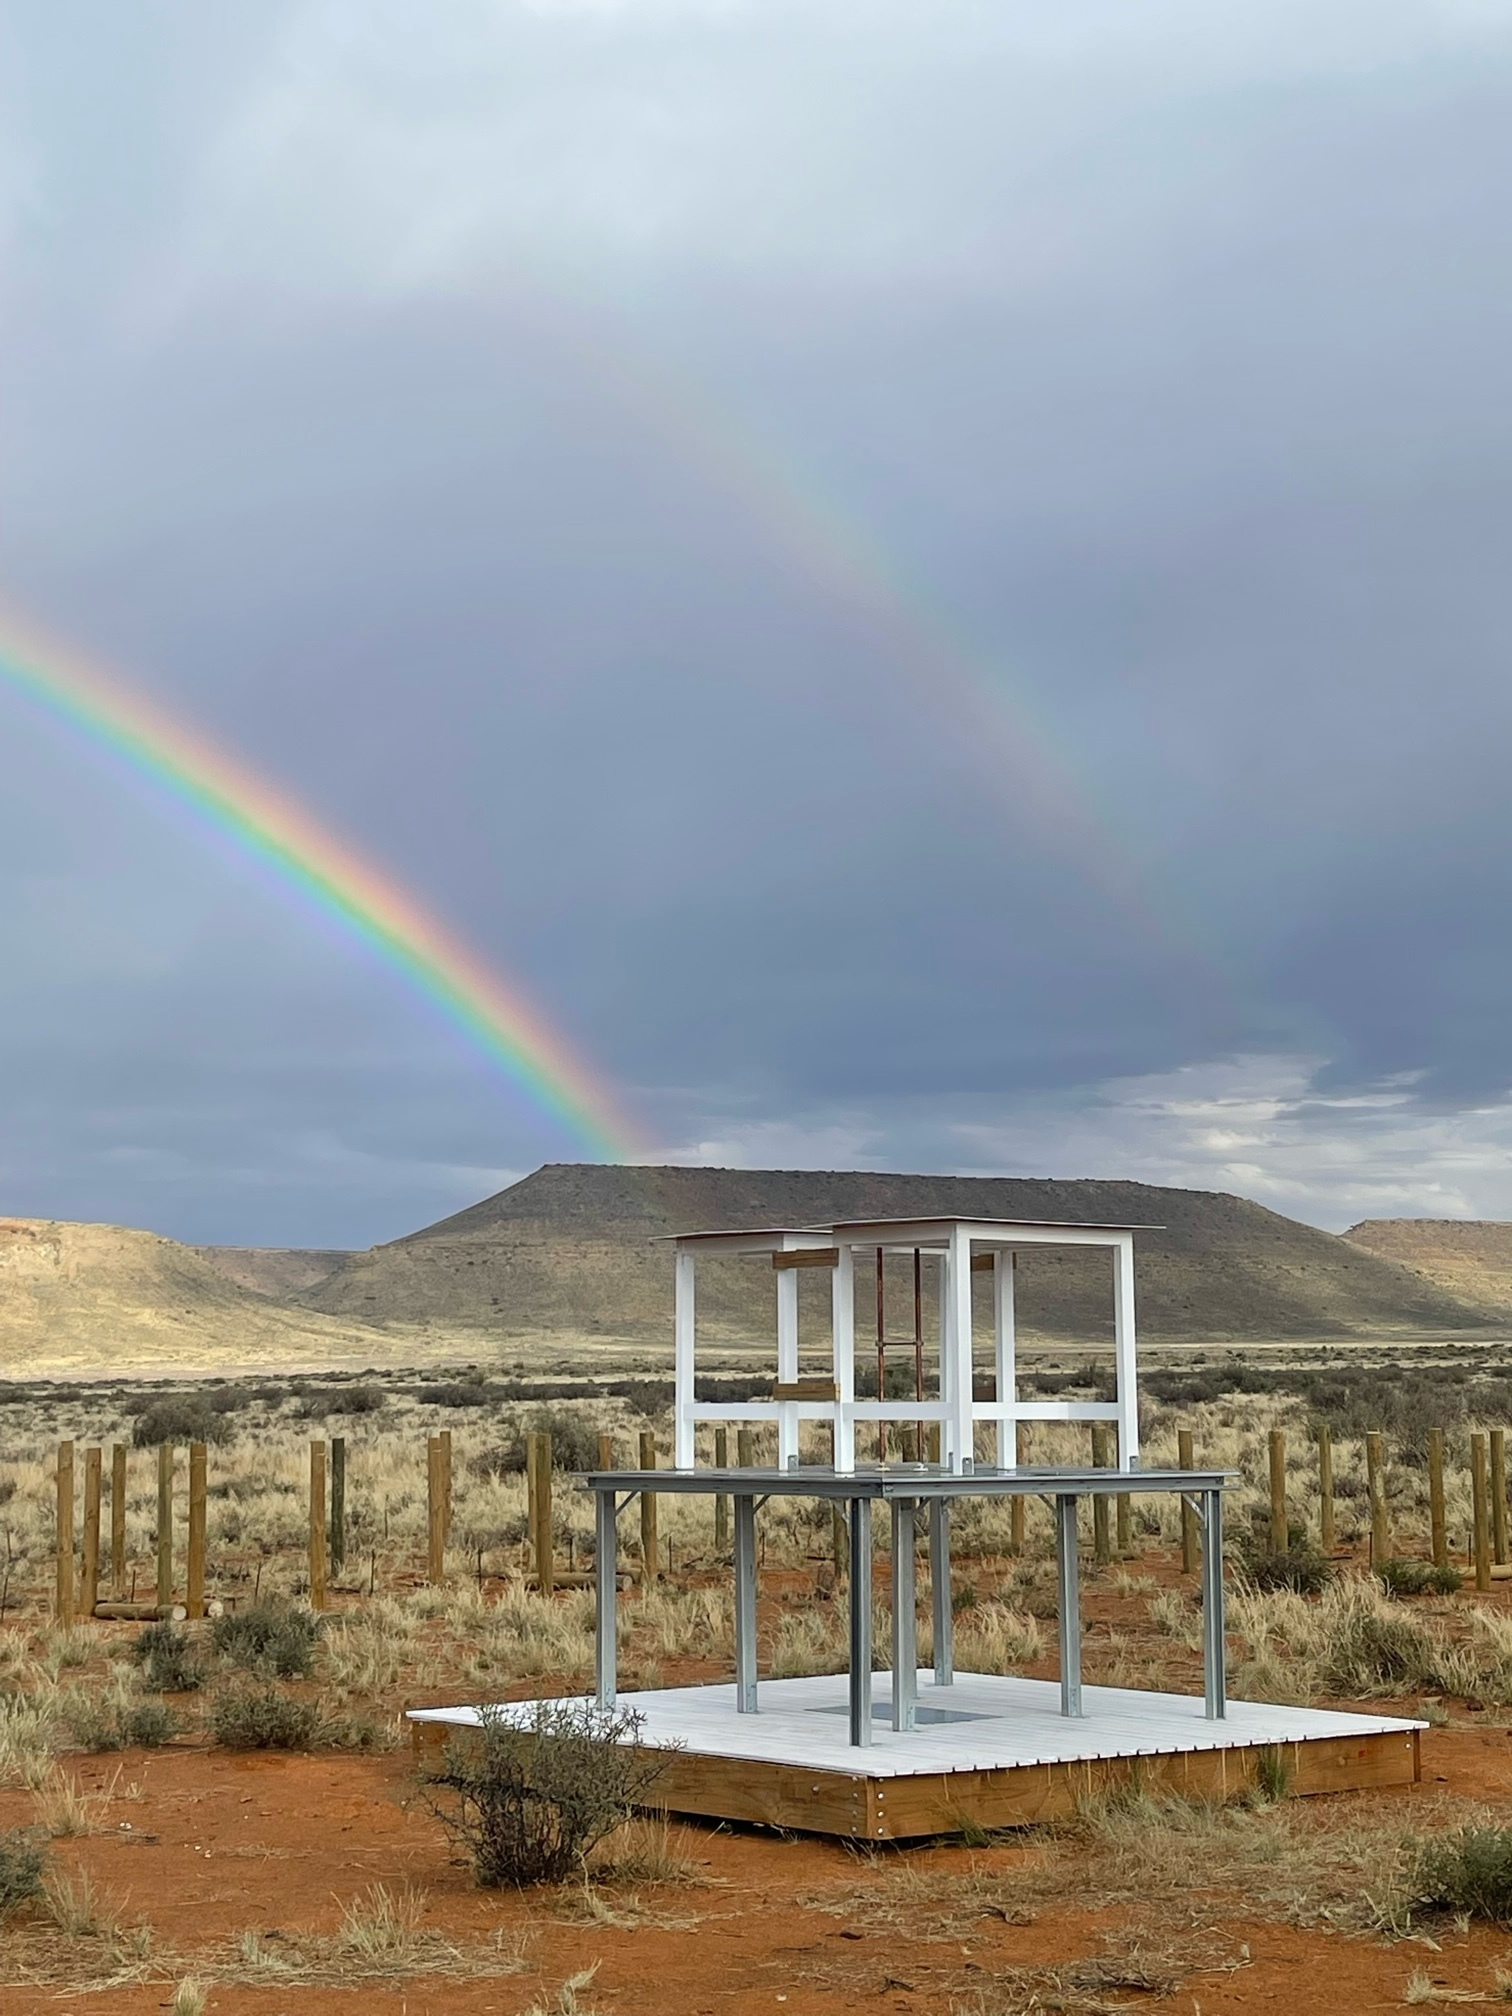
\includegraphics[height=0.3\textwidth]{figures/REACH_2.jpg}
        \end{itemize}
        \column{0.35\textwidth}
        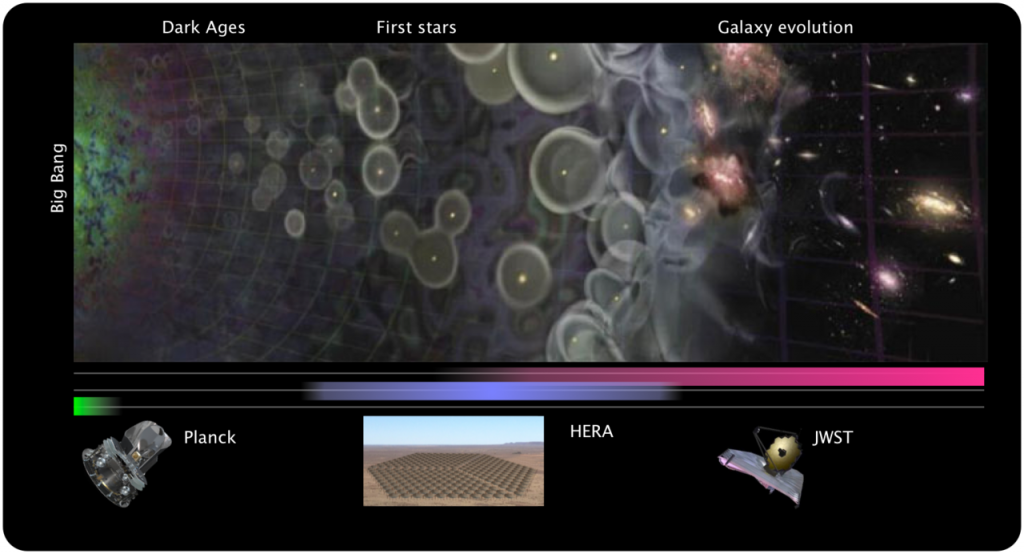
\includegraphics[width=\textwidth]{figures/21cm_1.png}
        \includegraphics[width=\textwidth]{figures/21cm.png}
    \end{columns}
\end{frame}

\begin{frame}
    \frametitle{GAMBIT: combining particle physics \& cosmological data}
    \begin{columns}
        \column{0.52\textwidth}
        \begin{itemize}
            \item Multinational team of particle physicists, cosmologists and statisticians.
            \item Combine cosmological data, particle colliders, direct detection, \& neutrino detectors in a statistically principled manner~\arxiv{2205.13549}.
            \item Lead Cosmo/Dark Matter working group~\arxiv{2009.03286}.
            \item Nested sampling used for global fitting, and fine-tuning quantification~\arxiv{2101.00428}
        \end{itemize}
        \begin{center}
            \includegraphics[width=0.5\textwidth]{figures/gambit_logo.png}
        \end{center}
        \column{0.48\textwidth}
        \vspace{-40pt}
        \includegraphics[width=\textwidth]{figures/ALP_2.pdf}
    \end{columns}
\end{frame}

\begin{frame}
    \frametitle{SBI: Simulation-based inference}
    \begin{columns}
        \column{0.5\textwidth}
        \begin{itemize}
            \item What do you do if you don't know \C[2]{$\mathcal{L}(D|\theta)$}?
            \item If you have a simulator/forward model $\theta \rightarrow D$
                defines an \C[2]{\emph{implicit} likelihood~$\mathcal{L}$}.
            \item Simulator generates samples from $\C[2]{\mathcal{L}(\cdot|\theta)}$.
            \item With a prior $\C[1]{\pi}(\theta)$ can generate samples from \C[4]{joint distribution}~$\C[4]{\mathcal{J}(\theta,D)}=\C[2]{\mathcal{L}(D|\theta)}\C[1]{\pi(\theta)}$\\\hfill \emph{the ``probability of everything''}.
            \item Task of SBI is take joint~$\C[4]{\mathcal{J}}$ samples and learn \C[0]{posterior $\mathcal{P}(\theta|D)$} and \C[3]{evidence $\mathcal{Z}(D)$} \\\hfill and possibly \C[2]{likelihood $\mathcal{L}(D|\theta)$}.
            \item Present state of the art achieves this using \emph{machine learning} (neural networks).
                \begin{itemize}
                    \item My group's research tries to removes machine learning \tthref{github.com/handley-lab/lsbi}.

                \end{itemize}
            %\item Present SotA: NPE, NLE, NJE, NRE
            %\item SBI \& forward modelling force us to think about data space~$D$ \& parameter space~$\theta$.
        \end{itemize}
        \column{0.5\textwidth}
        \includegraphics<1>[page=1, width=\textwidth]{figures/sbi_parameter_estimation.pdf}%
        \includegraphics<2>[page=2, width=\textwidth]{figures/sbi_parameter_estimation.pdf}%
        \includegraphics<3>[page=3, width=\textwidth]{figures/sbi_parameter_estimation.pdf}%
        \includegraphics<4>[page=4, width=\textwidth]{figures/sbi_parameter_estimation.pdf}%
        \includegraphics<5>[page=5, width=\textwidth]{figures/sbi_parameter_estimation.pdf}%
        \includegraphics<6>[page=6, width=\textwidth]{figures/sbi_parameter_estimation.pdf}%
        \includegraphics<7>[page=7, width=\textwidth]{figures/sbi_parameter_estimation.pdf}%
        \includegraphics<8>[page=8, width=\textwidth]{figures/sbi_parameter_estimation.pdf}%
        \includegraphics<9>[page=9, width=\textwidth]{figures/sbi_parameter_estimation.pdf}%
        \includegraphics<10>[page=10, width=\textwidth]{figures/sbi_parameter_estimation.pdf}%
        \includegraphics<11>[page=11, width=\textwidth]{figures/sbi_parameter_estimation.pdf}%
        \includegraphics<12>[page=12, width=\textwidth]{figures/sbi_parameter_estimation.pdf}%
        \includegraphics<13>[page=13, width=\textwidth]{figures/sbi_parameter_estimation.pdf}%
        \includegraphics<14>[page=14, width=\textwidth]{figures/sbi_parameter_estimation.pdf}%
        \includegraphics<15>[page=15, width=\textwidth]{figures/sbi_parameter_estimation.pdf}%
        \includegraphics<16>[page=16, width=\textwidth]{figures/sbi_parameter_estimation.pdf}%
        \includegraphics<17>[page=17, width=\textwidth]{figures/sbi_parameter_estimation.pdf}%
        \includegraphics<18>[page=18, width=\textwidth]{figures/sbi_parameter_estimation.pdf}%
        \includegraphics<19>[page=19, width=\textwidth]{figures/sbi_parameter_estimation.pdf}%
        \includegraphics<20>[page=20, width=\textwidth]{figures/sbi_parameter_estimation.pdf}%
        \includegraphics<21>[page=21, width=\textwidth]{figures/sbi_parameter_estimation.pdf}%
    \end{columns}
\end{frame}


\begin{frame}
    \frametitle{Neural Ratio Estimation}
    \begin{columns}
        \column{0.5\textwidth}
        \begin{itemize}
            \item SBI flavours: {\small \hfill\tthref{github.com/sbi-dev/sbi}}
                {\small
                    \begin{description}
                        \item[NPE] Neural posterior estimation
                        \item[NLE] Neural likelihood estimation
                        \item[NJE] Neural joint estimation
                        \item[NRE] Neural ratio estimation
                    \end{description}
                }
            \item NRE recap:
                \begin{enumerate}
                    \item Generate joint samples $(\theta,D)\sim\C[4]{\mathcal{J}}$
                        \label{step:joint}
                        \begin{itemize}
                            \item \textit{straightforward if you have a simulator:\\ $\theta\sim\C[1]{\pi(\cdot)}$, $D\sim\C[2]{\mathcal{L}(\cdot|\theta)}$}
                        \end{itemize}
                    \item Generate separated samples $\theta\sim\C[1]{\pi}$, $D\sim\C[3]{\mathcal{Z}}$\label{step:sep}
                        \begin{itemize}
                            \item \textit{aside: can shortcut step~\ref{step:sep} by scrambling the $(\theta,D)$ pairings from step~\ref{step:joint}}
                        \end{itemize}
                    \item Train probabilistic classifier $p$ to distinguish whether $(\theta,D)$ came from $\C[4]{\mathcal{J}}$ or $\C[1]{\pi}\times\C[3]{\mathcal{Z}}$.
                    \item $\frac{p}{1-p} = \C[5]{r} = \frac{P(\theta,D)}{P(\theta)P(D)} 
                        =
                        \frac{\C[4]{\mathcal{J}}}{\C[1]{\pi}\times\C[3]{\mathcal{Z}}} = \frac{\C[2]{\mathcal{L}}}{\C[3]{\mathcal{Z}}} = \frac{\C[0]{\mathcal{P}}}{\C[1]{\pi}}$.
                    \item Use ratio $\C[5]{r}$ for parameter estimation $\C[0]{\mathcal{P}} = \C[5]{r}\C[1]\times {\pi}$
                \end{enumerate}
        \end{itemize}
        \column{0.5\textwidth}
        \only<1|handout:0>{
            \begin{tikzpicture}[node distance=1cm, every neuron/.style={circle, draw, minimum size=1cm},]
                \node[every neuron/.try] (j2)  {};
                \node[every neuron/.try, above left = 0cm and 0.5cm of j2] (theta) { $\theta$};
                \node[every neuron/.try, below left = 0cm and 0.5cm of j2] (D) { $D$};
                \node[every neuron/.try, above = 0.5cm of j2] (j1) {};
                \node[every neuron/.try, below = 0.5cm of j2] (j3) {};
                \node[every neuron/.try, above right = 0cm and 0.5cm of j2] (h1) {};
                \node[every neuron/.try, below right = 0cm and 0.5cm of j2] (h2) {};
                \node[every neuron/.try, right = 1.3cm of j2] (p) { $p$};
                \node[every neuron/.try, right = 0.5cm of p] (logr) { $\C[5]{r}$};
                \draw[-] (theta) -- (j1);
                \draw[-] (D) -- (j1);
                \draw[-] (theta) -- (j2);
                \draw[-] (D) -- (j2);
                \draw[-] (theta) -- (j3);
                \draw[-] (D) -- (j3);
                \draw[-] (j1) -- (h1);
                \draw[-] (j1) -- (h2);
                \draw[-] (j2) -- (h1);
                \draw[-] (j2) -- (h2);
                \draw[-] (j3) -- (h1);
                \draw[-] (j3) -- (h2);
                \draw[-] (h1) -- (p);
                \draw[-] (h2) -- (p);
                \draw[-] (p) -- (logr);
                \node[below =0.5cm of logr] {\includegraphics[page=22, width=0.5\textwidth]{figures/sbi_parameter_estimation.pdf}};
            \end{tikzpicture}
        }
        \only<2>{
            \begin{exampleblock}{Bayesian proof}
                \begin{itemize}
                    \item Let $M_{\C[4]{\mathcal{J}}}$: $(\theta,D)\sim\C[4]{\mathcal{J}}$, $M_{\C[1]{\pi}\C[3]{\mathcal{Z}}}$: $(\theta,D)\sim\C[1]{\pi}\times\C[3]{\mathcal{Z}}$
                    \item Classifier gives
                        ${p(\theta,D) = P(M_{\C[4]{\mathcal{J}}}|\theta,D) = 1- P(M_{\C[1]{\pi}\C[3]{\mathcal{Z}}}|\theta,D)}$
                    \item Bayes theorem then shows
                        ${\frac{p}{1-p}=\frac{P(M_{\C[4]{\mathcal{J}}}|\theta,D)}{P(M_{\C[1]{\pi}\C[3]{\mathcal{Z}}}|\theta,D)} = \frac{P(\theta,D|M_{\C[4]{\mathcal{J}}})P(M_{\C[4]{\mathcal{J}}})}{P(\theta,D|M_{\C[1]{\pi}\C[3]{\mathcal{Z}}})P(M_{\C[1]{\pi}\C[3]{\mathcal{Z}}})} = 
                        \frac{\C[4]{\mathcal{J}}}{\C[1]{\pi}\C[3]{\mathcal{Z}}}}$, \\
                        where we have assumed 
                        \begin{itemize}
                            \item $P(M_{\C[4]{\mathcal{J}}}) = P(M_{\C[1]{\pi}\C[3]{\mathcal{Z}}})$,
                        \end{itemize}
                        and by definition
                        \begin{itemize}
                            \item $\C[4]{\mathcal{J}(\theta,D)} = P(\theta,D|M_{\C[4]{\mathcal{J}}})$
                            \item $\C[1]{\pi(\theta)}\C[3]{\mathcal{Z}(D)} = P(\theta,D|M_{\C[1]{\pi}\C[3]{\mathcal{Z}}})$.
                        \end{itemize}
                \end{itemize}
            \end{exampleblock}
        }
        \only<3|handout:0>{
            \begin{block}{Why I like NRE}
                \begin{itemize}
                    \item The link between classification and inference is profound.
                    \item Density estimation is hard -- Dimensionless $r$ divides out the hard-to-calculate parts.
                \end{itemize}
            \end{block}
            \begin{block}{Why I don't like NRE}
                \begin{itemize}
                    \item Practical implementations require marginalisation~\arxiv{2107.01214}, or autoregression~\arxiv{2308.08597}.
                    \item Model comparison and parameter estimation are separate~\arxiv{2305.11241}.
                \end{itemize}
            \end{block}
        }
    \end{columns}
\end{frame}

\begin{frame}
    \frametitle{TMNRE: Truncated Marginal Neural Ratio Estimation}
    \framesubtitle{\texttt{swyft}: \tthref{github.com/undark-lab/swyft}}
    \begin{columns}
        \column{0.55\textwidth}
        \begin{itemize}
            \item Two tricks for practical NRE:
        \end{itemize}
        \begin{block}{Marginalisation}
            \begin{itemize}
                \item Only consider one or two parameters at a time.
                \item Fine if your goal is to produce triangle plots.
                \item Problematic if information is contained jointly in more than two parameters.
            \end{itemize}
        \end{block}
        \begin{block}{Truncation}
            \begin{itemize}
                \item focus parameters $\theta$ on a subset of the prior which reproduces observed data $D_\text{obs}$
                \item region is somewhat arbitrary (usually a box)
                \item not amortised, sounds a bit like ABC
            \end{itemize}
        \end{block}
        \column{0.45\textwidth}
        \begin{overpic}[width=\textwidth]{figures/tmnre}
            \put(70,0) {\arxiv{2111.08030}}
        \end{overpic}
    \end{columns}
\end{frame}


\begin{frame}
    \frametitle{Similarities}
    \begin{columns}
        \column{0.5\textwidth}
        \includegraphics[width=\textwidth,page=15]{figures/himmelblau}% 
        \column{0.5\textwidth}
        \includegraphics[width=\textwidth]{figures/tmnre.pdf}
    \end{columns}
\end{frame}

\begin{frame}
    \frametitle{Sequential NRE with nested sampling}
    \begin{tikzpicture}[
            node distance=1cm,
            >=stealth, auto,
            every state/.style={
                rectangle, rounded corners, minimum width=2em,
                text width=6.8cm, align=center
            }
        ]
        \node[state, fill=C3!20, minimum height=3cm] (q14) {
            \textbf{NS}\\
            Run nested sampling on $\log r_{i}(\theta, D_\text{obs})$ \\
            to generate $\theta$ dead samples between prior and posterior targeted at $D_\text{obs}$.
        };
        \node[state, fill=C0!20, minimum height=1cm] (q121) [above=of q14] {
            \textbf{Terminate} if $\mathcal{D}_\text{KL}$ has converged
        };
        \node[state, fill=C0!20, minimum height=1cm] (q12) [above=of q121] {
            \textbf{Initialise} $\theta\sim\pi$\\
        };
        \node[state, fill=C2!20, minimum height=3cm] (q34) [right=of q14] {
            \textbf{NRE}\\
            Train Neural ratio estimator $\log r_i$
            with weights initialised from previous run
        };
        \node[state, fill=C1!20, minimum height=3cm] (q23) [above=of q34] {
            \textbf{Simulate}\\
            Generate simulations $\theta\to D$ from all discarded points
        };
        \begin{scope}[bend left]%
            \path[thick,-{Latex[width=2mm]}]   (q14.north) edge node {} (q121.south)
            (q121.east) edge node {}($(q23.south west)!0.16!(q23.north west)$) 
            (q23.south) edge node {} (q34.north)
            (q34.west) edge node {} (q14.east)
            (q12.east) edge node {}($(q23.south west)!0.84!(q23.north west)$) ;
        \end{scope}
        \node[align=center] (e) at (barycentric cs:q121=0.5,q12=0.5,q23=1,q34=1,q14=1) {\Large\textbf{NSNRE}};
    \end{tikzpicture}
\end{frame}

\begin{frame}
    \frametitle{\texttt{PolySwyft}}
    \begin{columns}[t]
        \column{0.45\textwidth}
        \begin{block}{\texttt{PolyChord}}
            \tthref{github.com/PolyChord/PolyChordLite}
            \includegraphics[width=\textwidth]{figures/polychord.png}
            \begin{itemize}
                \item Widely used high-performance nested sampling tool (implementing slice sampling \& clustering in MPI Fortran)
            \end{itemize}
        \end{block}
        \column{0.45\textwidth}
        \begin{block}{\texttt{Swyft}}
            \tthref{github.com/undark-lab/swyft}
            \includegraphics[width=\textwidth]{figures/swyft_logo_wide.png}
            \begin{itemize}
                \item Widely used TMNRE tool in cosmology/astrophysics.
            \end{itemize}
        \end{block}
        However, NSNRE is general, and not specific to these choices.
    \end{columns}
\end{frame}

\begin{frame}
    \frametitle{Convergence diagnostics}
    \begin{columns}
        \column{0.5\textwidth}
        \begin{itemize}
            \item Example for a $n=5$ dimensional parameter space, with $d=100$ data points, (\texttt{lsbi} gaussian mixture model).
            \item This is the regime for cosmological scale problems.
            \item To determine convergence we track:
                \begin{itemize}
                    \item The change in KL divergence between rounds (\C[0]{blue}), and check when this goes to zero.
                    \item The total KL divergence between prior and posterior estimate (\C[1]{orange}), and check when this levels off (ground truth in \C[3]{red}).
                    \item Also shown is the KL divergence between the estimate and the ground truth (\C[2]{green}).
                \end{itemize}
        \end{itemize}
        \column{0.5\textwidth}
        \includegraphics<1>[width=\textwidth]{figures/GMM_posterior_estimates.pdf}%
        \includegraphics<2|handout:0>[width=\textwidth]{figures/GMM_KL_div_per_round.pdf}
    \end{columns}
\end{frame}

\begin{frame}
    \frametitle{Posterior repartitioning}
    \student{aleksandr_petrosyan}{Aleksandr Petrosyan}{MSci 2021}
    \begin{columns}
        \column{0.5\textwidth}
        \begin{itemize}
            \item Almost all sampling algorithms (MH, HMC, SMC) are only sensitive to the product of likelihood and prior $\boxed{\C[2]{\mathcal{L}}\times\C[1]{\pi}}$.
            \item In practice this manifests as many codes implementing ``prior terms'' in the likelihood (or visa-versa) with no ill effect
        \item Nested sampling is unusual, in that one ``samples from the prior $\C[1]{\pi}$, subject to a hard constraint $\C[2]{\mathcal{L}}>\C[2]{\mathcal{L}_*}$.'':
                \[\{\theta\sim \C[1]{\pi} : \C[2]{\mathcal{L}}(\theta)>\C[2]{\mathcal{L}_*} \}\] 
            \item This separates the prior from the likelihood at an algorithmic level.
        \end{itemize}
        \column{0.5\textwidth}
        \begin{itemize}
\item One can therefore repartition the likelihood and prior $(\C[2]{\mathcal{L}},\C[1]{\pi})\to(\C[2]{\tilde{\mathcal{L}}},\C[1]{\tilde{\pi}})$, providing
                \[ \boxed{\C[2]{\mathcal{L}}\times\C[1]{\pi} = \C[2]{\tilde{\mathcal{L}}}\times\C[1]{\tilde{\pi}}}\]
            \item This moves pieces between likelihood and prior that you have analytic control over.
                \includegraphics[width=\textwidth]{figures/repartition}
            \item Chen, Feroz \& Hobson~\arxiv{1908.04655} invented this to deal with misspecified priors
        \end{itemize}
    \end{columns}
\end{frame}

\begin{frame}
    \frametitle{Posterior repartitioning for acceleration}
    \student{metha_prathaban}{Metha Prathaban}{PhD}
    \begin{columns}
        \column{0.5\textwidth}
        \begin{exampleblock}{Key idea}
Whilst posteriors and evidences are invariant to repartitioning $\C[2]{\mathcal{L}}\to\C[2]{\tilde{\mathcal{L}}}$, the KL divergence is not.
        \end{exampleblock}
    \begin{itemize}
            \item For constant ``run quality'' $\sigma$, 
            \begin{gather*} 
                {\scriptstyle
                    T = T_{\C[2]{\mathcal{L}}} \times n_\text{live} \times \mathcal{D}_\text{KL} \times f_\text{sampler}, \quad
\sigma \approx \sqrt{\mathcal{D}_\text{KL}/n_\text{live}} }
    \\
\Rightarrow\boxed{T = T_{\C[2]{\mathcal{L}}} \times \sigma \times \mathcal{D}_\text{KL}^2 \times f_\text{sampler}} 
        \end{gather*}
            so if you can reduce the KL divergence, then quadratic gains to be made
        \item \texttt{SuperNest}~\arxiv{2212.01760}
        \item Ongoing work with Metha Prathaban \& Harry Bevins.
    \end{itemize}
        \column{0.5\textwidth}
        \vspace{8pt}
        \includegraphics[width=\textwidth]{figures/supernest.pdf}
        \begin{itemize}
            \item Easy to get 40x performance normalised speed-up on cosmological scale cases
            \item Paper $\sim\mathcal{O}(\text{next month})$.
        \end{itemize}
    \end{columns}
\end{frame}

\begin{frame}
    \frametitle{Conclusions}
    \framesubtitle{\tthref{github.com/handley-lab}}
    \tikz[overlay,remember picture]
        \node[anchor=north east] (A) at ($(current page.north east)+(0,0)$) {
        \includegraphics[width=0.09\textheight]{figures/students/adam_ormondroyd.jpg}%
        \includegraphics[width=0.09\textheight]{figures/students/charlotte_priestley.jpg}%
        \includegraphics[width=0.09\textheight]{figures/students/david_yallup.jpg}%
        \includegraphics[width=0.09\textheight]{figures/students/dily_ong.jpg}%
        \includegraphics[width=0.09\textheight]{figures/students/george_carter.jpg}%
        \includegraphics[width=0.09\textheight]{figures/students/harry_bevins.jpg}%
        \includegraphics[width=0.09\textheight]{figures/students/ian_roque.jpg}%
        \includegraphics[width=0.09\textheight]{figures/students/kilian_scheutwinkel.jpg}%
        \includegraphics[width=0.09\textheight]{figures/students/metha_prathaban.jpg}%
        \includegraphics[width=0.09\textheight]{figures/students/namu_kroupa.jpg}%
        \includegraphics[width=0.09\textheight]{figures/students/sinah_legner.jpg}%
        \includegraphics[width=0.09\textheight]{figures/students/sam_leeney.jpg}%
        \includegraphics[width=0.09\textheight]{figures/students/thomas_gessey-jones.jpg}%
        \includegraphics[width=0.09\textheight]{figures/students/wei-ning_deng.jpg}%
    };
    \vspace{-0.1\textheight}
    \begin{columns}
        \column{0.65\textwidth}
    \begin{itemize}
        \item Nested sampling is a multi-purpose numerical tool for:
            \begin{itemize}
                \item Numerical integration $\int f(x) dV$,
                \item Exploring/scanning/optimising \textit{a priori} unknown functions,
                \item Performing Bayesian inference and model comparison.
            \end{itemize}
        \item It is applied widely across cosmology, particle physics \& machine learning.
        \item It's unique traits as the only numerical Lebesgue integrator mean with compute it will continue to grow in importance.
    \end{itemize}
        \column{0.35\textwidth}
    \includegraphics[height=0.6\textwidth]{figures/pps_both}%
    \includegraphics[height=0.6\textwidth]{figures/REACH_2}%
    \end{columns}
    \includegraphics[height=0.2\textwidth]{figures/integration}%
    \includegraphics[height=0.2\textwidth]{figures/curvature_3}%
    \includegraphics[height=0.2\textwidth]{figures/ALP_3}%
\end{frame}



\appendix

\end{document}
